\documentclass[11pt,a4paper]{article}
\usepackage[T1]{fontenc}
\usepackage{lmodern}
\usepackage[margin=27mm]{geometry}
\usepackage{amsmath,amssymb,amsthm,mathtools}
\usepackage{graphicx,booktabs,longtable,array,tabularx,multirow}
\newcolumntype{P}[1]{>{\raggedright\arraybackslash}p{#1}}
\renewcommand{\tabularxcolumn}[1]{P{#1}}
\usepackage[table]{xcolor}
\usepackage{microtype}
\usepackage{enumitem}
\usepackage{caption,subcaption}
\usepackage[section]{placeins}
\usepackage[numbers,sort&compress]{natbib}
\usepackage{xurl}
\usepackage[colorlinks=true,linkcolor=blue!45!black,citecolor=blue!45!black,urlcolor=blue!45!black]{hyperref}
\hypersetup{pdftitle={Kobon Triangle Constructions: Uniform Lower Bounds, Extension Methods, and Formal Verification},pdfauthor={Alejandro Zarzuelo Urdiales},pdfsubject={Research manuscript with exact certificates and Lean proof scope}}
\usepackage[nameinlink,noabbrev]{cleveref}
\usepackage{listings}
\usepackage{fancyhdr}
\setlength{\headheight}{14pt}
\pagestyle{fancy}
\fancyhf{}
\fancyhead[L]{\small Kobon triangle constructions and formal verification}
\fancyhead[R]{\small A. Zarzuelo Urdiales}
\fancyfoot[C]{\thepage}
\renewcommand{\headrulewidth}{0.25pt}
\setlength{\emergencystretch}{2em}
\setlength{\parskip}{3pt}
\setlist{itemsep=2pt,topsep=4pt}
\captionsetup{font=small,labelfont=bf,margin=5mm}
\setcounter{topnumber}{3}
\setcounter{bottomnumber}{2}
\setcounter{totalnumber}{5}
\renewcommand{\topfraction}{0.92}
\renewcommand{\bottomfraction}{0.85}
\renewcommand{\textfraction}{0.07}
\renewcommand{\floatpagefraction}{0.7}
\graphicspath{{figures/}}
\newtheorem{theorem}{Theorem}[section]
\newtheorem{proposition}[theorem]{Proposition}
\newtheorem{lemma}[theorem]{Lemma}
\newtheorem{corollary}[theorem]{Corollary}
\theoremstyle{definition}
\newtheorem{definition}[theorem]{Definition}
\newtheorem{conjecture}[theorem]{Conjecture}
\theoremstyle{remark}
\newtheorem{remark}[theorem]{Remark}
\newcommand{\K}{K}
\newcommand{\Ks}{K_{\mathrm{s}}}
\newcommand{\G}{G}
\newcommand{\B}{B}
\newcommand{\N}{\mathbb{N}}
\newcommand{\R}{\mathbb{R}}
\newcommand{\Z}{\mathbb{Z}}
\newcommand{\U}{U}
\newcommand{\Lbound}{L}
\newcommand{\floor}[1]{\left\lfloor#1\right\rfloor}
\newcommand{\ceil}[1]{\left\lceil#1\right\rceil}
\newcommand{\lean}[1]{{\small\nolinkurl{#1}}}
\newcommand{\repo}{\url{https://github.com/alejandrozu/kobon-proof}}
\newcommand{\status}[1]{\textsf{\small[#1]}}
\DeclareMathOperator{\sgn}{sgn}
\DeclareMathOperator{\conv}{conv}
\DeclareMathOperator{\intt}{int}
\lstset{basicstyle=\ttfamily\footnotesize,breaklines=true,columns=fullflexible,keepspaces=true,frame=single,framerule=0.3pt,rulecolor=\color{black!25},xleftmargin=4pt,xrightmargin=4pt}
\title{Kobon Triangle Constructions:\\Uniform Lower Bounds, Extension Methods,\\and Formal Verification}
\author{Alejandro Zarzuelo Urdiales}
\date{22 September 2026}
\begin{document}
\maketitle
\begin{abstract}
The Kobon triangle problem asks for the largest number of bounded triangular cells determined by a prescribed number of straight lines in the real affine plane. We give a unified account of a construction and verification program begun in March 2026, distinguishing completed geometric theorems, exact finite certificates, conditional families, and unresolved extension claims. The principal completed all-order result is a simple-line construction with at least $\floor{n(n-3)/3}+1+(n\bmod2)$ triangles for every $n\ge4$, together with the elementary smaller cases. A phase refinement and changes of affine chart supply a constant-term improvement of the familiar F\"uredi--Pal\'asti lower formula. We prove its geometry and counting in Lean and combine it with 138 exact finite certificates, retaining the authorship of published inputs. Further results include a verified exterior-line construction, an obstruction to unrestricted repetition of full exterior gains, a geometric one-step specialization of Bartholdi--Blanc--Loisel doubling, and local multiplicity-sensitive lemmas for upper-bound arguments. We document the earlier values at 28, 30 and 34 lines, the finite and proposed infinite families, unsuccessful searches, and the precise remaining proof obligations. The affine numerical refinement is compared carefully with the original projective counts and stronger published subsequences; numerical first priority and an unrestricted successor theorem are not asserted. All figures are generated anew from recorded formulas, coordinates, or experiments.
\end{abstract}
\vspace{0.4em}
\noindent\textbf{Keywords.} Line arrangements; triangular cells; Kobon problem; constructive lower bounds; projective transformations; exact computation; Lean formalization.
\clearpage
\tableofcontents
\clearpage
\section{Introduction and scope of the results}\label{sec:introduction}

An arrangement of $n$ straight lines divides the real plane into bounded and unbounded cells. The Kobon problem asks how many of the bounded cells can be triangles. The difficulty is not creating many triples of intersecting lines: there are $\binom n3$ candidate triples. The difficulty is ensuring that their triangles are not cut by any of the remaining lines and that their interiors do not overlap. The distinction between an attractive picture and a valid arrangement is therefore central to both construction and verification.

Let $\K(n)$ denote the classical maximum, allowing multiple intersections and parallel lines, and let $\Ks(n)$ denote the maximum over simple arrangements: no parallel pair and no three concurrent lines. All lower-bound witnesses constructed by the universal theorem below are simple, so they establish lower bounds for both quantities. Some of the strongest retained finite certificates are nonsimple. We never use an upper bound restricted to $\Ks$ as an upper bound for $\K$ without an additional argument.

This paper consolidates the author's March 2026 extension proposal and the subsequent program of exact construction, comparison with the literature, and formal proof. The purpose is both mathematical and documentary: to state the strongest completed results, to make their proofs and provenance inspectable, and to preserve the failed approaches that determine the next research questions. The original general extension claim is reported as an unresolved claim rather than silently promoted to a theorem.

\subsection{The main completed all-order theorem}

Define $\B(n)=\ceil{n(n-3)/3}$ for $n\ge3$, and set $\B(n)=0$ for $n<3$. The familiar F\"uredi--Pal\'asti construction supplies this affine baseline; the underlying construction and its historical priority belong to the earlier literature~\cite{furedipalasti1984,erickson1999}. Our principal completed theorem is the following refinement.

\begin{theorem}[Universal affine refinement]\label{thm:main}
For every $n\in\N$, there is a simple arrangement of $n$ real straight lines with at least $\G(n)$ bounded triangular cells, where
\begin{equation}\label{eq:G}
\G(n)=\begin{cases}
0,&0\le n<3,\\
1,&n=3,\\
\floor{n(n-3)/3}+1+(n\bmod2),&n\ge4.
\end{cases}
\end{equation}
Consequently $\K(n)\ge\Ks(n)\ge\G(n)$.
\end{theorem}

The proof, developed in Section~\ref{sec:universal}, combines a shifted trigonometric arrangement with one- and two-cap changes of affine chart. The Lean declaration \lean{Kobon.Universal.baseline_sound} proves the geometric existence statement for arbitrary $n$. It has no assumed extension theorem and no dependence on finite experimental verification. Its dependencies are the standard logical axioms used by Lean and Mathlib.

For $n\ge4$, the gains over $\B(n)$ are $1,1,0,2,0,1$ in residue classes $0,1,2,3,4,5$ modulo six. Thus the refinement is strict at every odd order at least five and every positive multiple of six. Both formulas have leading behavior $n^2/3-n+O(1)$: this is a constant-term refinement, not an improved quadratic or linear asymptotic coefficient. The original F\"uredi--Pal\'asti projective count table already contains related constants. The present source audit does not establish first numerical priority for the affine formula.

\begin{figure}[tbp]
\centering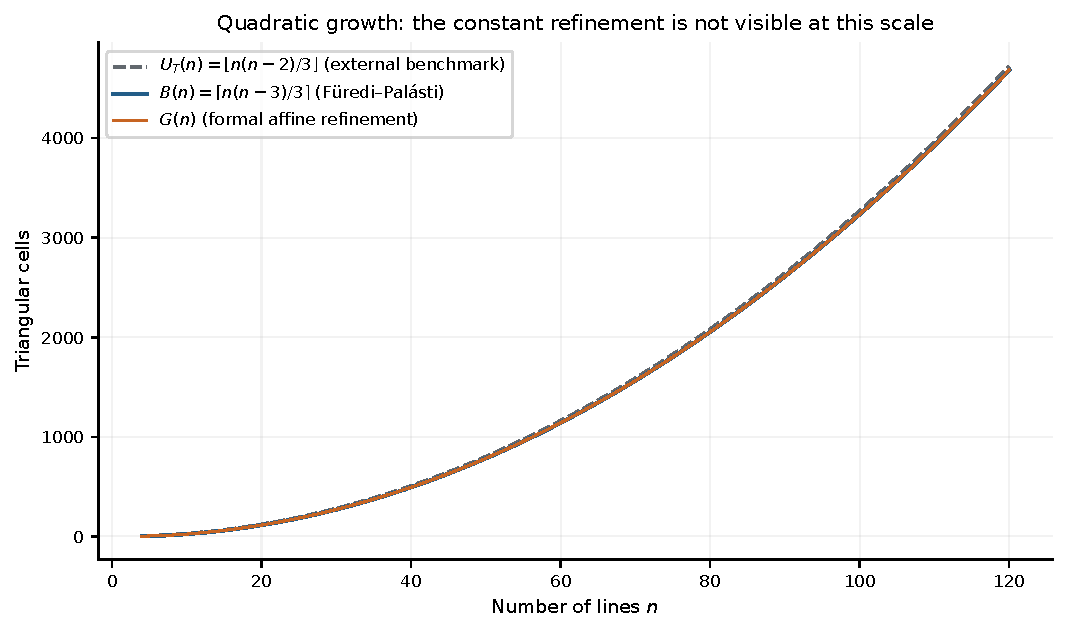
\includegraphics[width=0.94\linewidth]{bounds-growth.pdf}
\caption{Growth of the classical general baseline, the proved affine refinement, and the classical polynomial upper benchmark. The close overlap on a quadratic scale is mathematically meaningful: the new uniform gain is bounded. Residue and deficit plots below resolve the smaller differences. This figure is computed from the formulas, not copied from earlier publications.}\label{fig:growth}
\end{figure}

\subsection{Finite enhancements and other completed components}

The universal construction is supplemented by exact coordinates. Let $C(n)$ be the largest triangle count among the finite certificates in the release at order $n$, with $C(n)=0$ when no such certificate is saved. Then
\begin{equation}\label{eq:envelope}
\Lbound(n)=\max\{\G(n),C(n)\},\qquad \K(n)\ge\Lbound(n)
\end{equation}
is proved for all natural orders. This elementary maximum operation retains published constructions and the author's earlier values without altering their attribution. It is not a claim that $\Lbound$ is the largest lower bound obtainable from all published constructions by every possible interpolation or extension.

The finite catalog contains 138 distinct coordinate certificates, including 104 simple witnesses. A separate generated table has 64 orders at which a saved finite certificate strictly improves the older baseline $\B$; some of these improvements are already supplied by $\G$. The catalog includes weaker checkpoints and independent reproductions. Its size is not a count of original discoveries.

The other completed components are an actual exterior-line construction from certified visible pairs; a finite boundary-resource obstruction to repeatedly obtaining the full proposed successor gain; a geometric BBL doubling step under specified seed hypotheses; and local geometric lemmas about fans at multiple intersections. Their scope is summarized in Table~\ref{tab:claims}. The distinction between a proved local step and a recursively closed infinite family is maintained throughout.

\begin{table}[tbp]
\centering\small
\begin{tabularx}{\linewidth}{@{}P{0.28\linewidth}XP{0.21\linewidth}@{}}
\toprule
Result & Mathematical content & Release status\\
\midrule
Universal $\G$ & Simple real-line witnesses at every order & General Lean proof\\
Envelope $\Lbound$ & Maximum with all saved finite witnesses & Lean; finite native checks\\
28:238, 30:275, 34:357 & Earlier attributed finite inequalities & Exact Lean certificates\\
Exterior extension & New line and gain from a visible-pair list & General Lean proof\\
Full successor recurrence & $\K(n+1)\ge\K(n)+\floor{n/2}$ & Unproved\\
49-seed numerical target & Lower function obtained by summing the proposed recurrence & Independently proved\\
One-step BBL doubling & $(q+1,T)\mapsto(2q+1,T+q^2)$ for compatible seeds & General Lean proof\\
Infinite hybrid iteration & Preservation and repeated use of the seed invariant & Incomplete Lean integration\\
Local fan structure & Incidence, antipodal and run-length restrictions & General Lean proofs\\
Global multiplicity consequences & Upper-budget inequalities from geometric charging & Paper-level; bridge open\\
\bottomrule
\end{tabularx}
\caption{Claim status in the frozen mathematical release. ``General Lean proof'' does not imply that every proposed application has been formalized. Published construction inputs retain their original authorship.}\label{tab:claims}
\end{table}

\subsection{History, attribution, and the structure of the paper}

The March archive records a proposed extension from odd to even orders, associated finite bounds, and an incomplete Lean file. That file contains eight proof placeholders, including its central extension step. Later exact certificates establish the finite inequalities independently, while the current all-order proof uses a different construction. Accordingly, a corrected account must separate the survival of numerical conclusions from the validity of the original proof strategy.

The September work broadened the program to both parities, exterior visibility, boundary-defect estimates, compatible doubling seeds, exact rational realization, and multiplicity-sensitive upper arguments. Several plausible routes failed: direct repetition of exterior gains lost the necessary boundary resources; small perturbations of nonsimple records sometimes reduced the triangle count; and large local searches failed to improve their chosen seeds. These negative findings are recorded with their exact scope rather than converted into impossibility theorems.

Section~\ref{sec:geometry} states the geometric definitions and the certificate-to-cell bridge. Section~\ref{sec:universal} proves the uniform refinement; Section~\ref{sec:finite} records finite cases and provenance. The following sections develop extension and family results, local upper-bound ingredients, and computational searches. The final sections describe the formal trust boundary and future obligations. The appendices contain the complete finite tables and a map from mathematical claims to proof sources. The code and evidence are available at \repo~\cite{zarzueloRepository}.

\section{Literature, provenance, and the scope of comparison}
\label{lit:review}

\subsection{Four distinctions that affect every comparison}

The literature studies several related extremal functions. Their numerical tables cannot be combined without retaining their hypotheses. Throughout this paper, $\K(n)$ concerns straight lines in the real affine plane and permits multiple intersections and parallel pairs, whereas $\Ks(n)$ restricts to pairwise nonparallel lines with no three concurrent. Only bounded triangular cells are counted. A pseudoline arrangement is a topological relaxation; a lower bound obtained there becomes a straight-line lower bound only after realizability has been established. Finally, projective triangular faces need not remain bounded after an affine chart is chosen.

\begin{table}[htbp]
\centering\small
\begin{tabularx}{\textwidth}{@{}lXX@{}}
\toprule
Distinction & What transfers immediately & What requires another argument\\
\midrule
Simple / unrestricted & A simple example is an unrestricted example. & A simple upper bound need not bound a configuration with concurrent lines.\\
Straight / pseudoline & Every straight arrangement is a pseudoline arrangement. & A pseudoline construction requires a straight realization.\\
Affine / projective & Projective transformations preserve incidence and projective faces. & Boundedness depends on the line chosen as infinity.\\
Finite / infinite & A certified configuration proves its individual lower bound. & Iteration requires the next configuration to satisfy every input invariant.\\
\bottomrule
\end{tabularx}
\caption{Logical distinctions used throughout the source audit.}
\label{lit:scope-table}
\end{table}

There are also two different projective-to-affine operations. Choosing a new line at infinity outside an $n$-line arrangement keeps $n$ lines, but may lose triangular faces to infinity. Making one of the arrangement's own lines the line at infinity and removing it produces an $(n-1)$-line affine arrangement. The latter operation underlies several optimal subsequences; the former is central to the uniform construction formalized here.

\subsection{From the puzzle to arrangement theory}

Fujimura's puzzle reached English readers through \emph{The Tokyo Puzzles}, edited by Gardner and translated by Adachi~\citep{fujimura1978}; Gardner also discussed it in his collected mathematical recreations~\citep{gardner1983}. The broader theory of line and pseudoline arrangements is developed in Gr\"unbaum's monograph~\citep{grunbaum1972}. The papers of Strommer and Purdy document an established extremal-triangle literature preceding the construction used in this paper~\citep{strommer1977,purdy1979,purdy1980}. We cite those early papers as historical context rather than silently identifying all their projective or non-simple questions with the affine function $\K$.

The familiar comparison polynomial is
\begin{equation}
 U_{\mathrm T}(n)=\left\lfloor\frac{n(n-2)}3\right\rfloor.
 \label{lit:tamura}
\end{equation}
The attribution to Saburo Tamura is transmitted in the Cl\'ement--Bader draft~\citep{clementbader2007}; an original publication by Tamura was not located in this audit. We therefore do not manufacture an independent bibliographic item for that attribution. Cl\'ement and Bader report the stronger classical envelope $U_{\mathrm T}(n)-1$ for $n\equiv0,2\pmod6$. Section~\ref{upper:scope} explains both the scope of this reported result and a local proof-reading issue. A source-reported upper bound and an upper bound proved in our Lean development are different kinds of evidence.

\subsection{The F\"uredi--Pal\'asti all-order construction}

F\"uredi and Pal\'asti gave highly triangular straight-line arrangements using trigonometric coordinates~\citep{furedipalasti1984}. Their projective Table~1 has a residue-dependent constant term. The familiar affine consequence is commonly written
\begin{equation}
 \B(n)=\left\lceil\frac{n(n-3)}3\right\rceil\qquad(n\ge3).
 \label{lit:baseline}
\end{equation}
Erickson states this formula explicitly in Section~7.2 while using arrangements in a computational-geometric lower-bound argument~\citep{erickson1999}. Felsner and Kriegel place the construction in the study of Euclidean triangular cells~\citep{felsnerkriegel1999}. A later discussion by Dam\'asdi, Mart\'inez-Sandoval, Nagy and Nagy quotes the slightly weaker floor version while studying triangle areas~\citep{damasdi2020}. Thus a general lower bound valid at every order existed well before the present work.

Our completed formula is
\begin{equation}
 \G(n)=\left\lfloor\frac{n(n-3)}3\right\rfloor+1+(n\bmod2),
 \qquad n\ge4.
 \label{lit:our-formula}
\end{equation}
The constructions in later sections prove this for actual simple affine lines. Table~\ref{lit:residue-comparison} separates its arithmetic improvement over~\eqref{lit:baseline} from the projective count in the original paper. Here $P_{\mathrm{FP}}(n)$ denotes the latter construction's projective count, not the projective maximum.

\begin{table}[htbp]
\centering\small
\begin{tabular}{@{}cclc@{}}
\toprule
$n\bmod6$ & $\G-\B$ & $P_{\mathrm{FP}}(n)$, $n\ge5$ & $P_{\mathrm{FP}}-\G$\\
\midrule
0 & 1 & $n(n-3)/3$ & $-1$\\
1 & 1 & $(n^2-3n+5)/3$ & $0$\\
2 & 0 & $(n^2-3n+8)/3$ & $2$\\
3 & 2 & $(n^2-3n+9)/3$ & $1$\\
4 & 0 & $(n^2-3n+8)/3$ & $2$\\
5 & 1 & $(n^2-3n+5)/3$ & $0$\\
\bottomrule
\end{tabular}
\caption{Exact comparison with the quoted affine baseline and with the original projective construction's face counts. A projective surplus does not itself supply additional bounded affine triangles.}
\label{lit:residue-comparison}
\end{table}

The numerical gain is bounded by two. In particular, the quadratic coefficient $1/3$ and linear coefficient $-1$ remain unchanged. What the completed proof adds is a phase refinement, a controlled choice of affine chart for odd orders, and an end-to-end geometric formalization. The audited sources do not provide an explicit statement of~\eqref{lit:our-formula} with this affine proof. That observation is not an exhaustive numerical-priority theorem: old projective constructions contain related counts, and an unnoticed affine-chart argument could have been available earlier. The defensible claim is the proved improvement over the explicitly quoted formula~\eqref{lit:baseline}, together with the formal construction; a claim of first numerical discovery is withheld.

\subsection{Optimal subsequences and the straightening problem}

Harborth and Roudneff developed constructions and extremal results for pseudolines~\citep{harborth1985,roudneff1996}. Their scope matters because topological realizability does not imply straight realizability. Forge and Ram\'irez Alfons\'in constructed a projective straight-line family at orders $2\cdot2^t+2$\citep{forge1998}. Removing a distinguished line at infinity gives optimal affine orders $2\cdot2^t+1$; in particular, this is the relevant older source for the $33$-line order.

Bartholdi, Blanc and Loisel's preprint appeared in 2007 and its proceedings publication in 2008~\citep{bbl2008}. Their compatible doubling step takes $q+1$ lines to $2q+1$ and adds $q^2$ triangles. It requires a prescribed tangent grid and a fully used distinguished line. Their straight-line optimal series include $14\cdot2^t+1$ and $6\cdot2^t+1$; their $18\cdot2^t+1$ series was then a pseudoline result. The general numerical recurrence is therefore prior work, not a new theorem of this project. Our contribution to that step is the verified real-coordinate specialization and its explicitly recorded hypotheses.

Parpalak and Utkin supplied a compatible straight $19$-line seed and established the straight-line series $n=18\cdot2^t+1$\citep{parpalakutkin2026}. Its triangle count is $108\cdot4^t-1$. Substitution into our formula gives the exact comparison
\begin{equation}
 \bigl(108\cdot4^t-1\bigr)-\G(18\cdot2^t+1)=6\cdot2^t-2.
 \label{lit:pu-gap}
\end{equation}
Thus their series is stronger at these orders: the comparisons begin $107>103$ at $19$, $431>421$ at $37$, and $1727>1705$ at $73$. Their separate even-series draft is also relevant prior construction evidence~\citep{parpalakutkinEven2026}. Its numerical families are not replaced by a weaker universal formula.

It would consequently be misleading to call $\G$ the strongest numerical lower bound for every $n$, or an unqualified state of the art among all possible all-order formulas. Taking a maximum with known special constructions already improves it. Padding a configuration by lines sufficiently far away preserves its bounded triangles and extends each special construction to later orders. The retained function in the repository likewise takes a maximum with its finite certificate catalogue. The purpose of $\G$ is a compact uniform guarantee with a complete formal proof, not the suppression of stronger special cases.

\subsection{Upper-bound refinements retain their simplicity assumptions}

The even-order bound
\[
 \left\lfloor\frac{n(n-7/3)}3\right\rfloor
\]
in Bartholdi--Blanc--Loisel applies to \emph{simple affine pseudoline} arrangements. Blanc subsequently proved the sharper common even-order polynomial
\begin{equation}
 \Ks(n)\le\left\lfloor\frac{n(n-5/2)}3\right\rfloor,
 \qquad n\text{ even},
 \label{lit:blanc-even}
\end{equation}
also in the simple pseudoline setting~\citep{blanc2011}. The latter work was posted in 2008 and published in 2011. Its parity argument is the starting point for our clean-line accounting outside a multiple-point core.

The distinction is concrete. Formula~\eqref{lit:blanc-even} equals $53$ at $n=14$, whereas a nonsimple configuration with $54$ triangles exists. Applying a simple upper theorem to that configuration would be invalid. Our upper-bound work therefore counts shared sides and multiple incidences explicitly rather than treating a small perturbation to general position as automatically harmless.

\subsection{Recent computational constructions and versioned claims}

Savchuk's 2025 work combines arrangement tables, SAT search, and heuristic straightening~\citep{savchuk2025}. It reports optimal $23$- and $27$-line configurations and an exclusion of a perfect $33$-triangle arrangement at order $11$. Its Appendix~A.4 records the earlier Honma-based $11$-line construction. For our purposes, an arrangement table, a floating-point fit, an exact straight-line certificate, and an exhaustive upper-bound exclusion are four different outputs. The present work independently verifies the coordinate lower bounds it imports; it does not thereby replay the external SAT exclusions.

Maiorana released fifteen exact $14$-line, $54$-triangle configurations~\citep{maiorana2026}. We preserve their attribution and the source's CC BY 4.0 license. The current Parpalak--Utkin gallery supplies further exact constructions, including nonsimple even-order examples~\citep{parpalakutkinGallery2026}. The $8$-line construction has earlier provenance; citing its current host does not transfer its invention to the host authors. Each retained dataset is tied to a source revision, checked independently, and distinguished from any stronger optimality language used in its original repository.

Versioning also matters for exclusions. The fourth version of Liang, Liu and Zhang's preprint concerns symmetry restrictions for simple $28$-line configurations~\citep{liangliuZhang2026}. It is not treated here as a proof of an unrestricted exact value, and its displayed numerical comparison is not substituted for Blanc's simple upper theorem. The ProofAtlas research page similarly reports restricted upper results while keeping the unrestricted problem open~\citep{proofatlas2026}. We record these as current research sources, not as independently reproduced proofs.

\subsection{The March result, later verification, and attribution}

The author's March manuscript proposed an even-order extension and recorded the values $238$, $275$, and $357$ at orders $28$, $30$, and $34$\citep{zarzuelo2026}. These values are now supported in this project by exact simple-line certificates. The associated original Lean file, however, contained placeholders, including the general extension lemma. The later successful formalizations do not retroactively turn that unfinished universal argument into a proof.

OEIS A006066 indexes numerical data, references, and named contributions~\citep{oeisA006066}. It is not a complete priority database. In particular, the 2007 Bartholdi--Blanc--Loisel table already contains a bold, hence straight-realizable, $30{:}275$ entry. The $34{:}357$ value follows from the older perfect $33$-line family and its exterior extension. At $28$ lines, Savchuk describes the analogous extension of the $27$-line solution. These overlaps require a distinction between an independently supplied construction, a new exact or formal certificate, and the first known numerical lower bound. We retain the author's recorded contribution without claiming first numerical priority solely from the OEIS attribution.

The recurrence reproduced by HandWiki~\citep{handwiki2026} is likewise a record of the proposed claim rather than a substitute for its proof. The unrestricted statement
\[
 \K(n+1)\ge\K(n)+\left\lfloor n/2\right\rfloor
\]
has not been established by the work reported here. What has been established includes a geometric exterior extension under explicit visibility hypotheses, finite successful successor steps, and a separate unconditional all-order construction. Their logical roles remain distinct.

\subsection{What formal verification contributes}

The proof infrastructure uses Lean~4~\citep{lean4} and mathlib~\citep{mathlib}. For the universal result, it connects analytic line equations, determinant signs, triangular cells, affine-chart control, and finite counting, rather than checking the final arithmetic formula in isolation. For finite results, it turns attributed coordinates into explicit certificates. For the upper-bound investigation, it proves local geometric and combinatorial lemmas while leaving the global arrangement extraction visibly unfinished.

The accompanying repository~\citep{zarzueloRepository} records source revisions, negative searches, axiom reports, and the boundary between proved statements and proposed research. This separation is part of the result: a complete formal proof of a modest uniform improvement is stronger evidence than an ambitious recurrence with an unproved geometric step. It does not by itself confer numerical priority or solve the unrestricted Kobon problem.

\section{Real-line geometry and exact certificates}\label{sec:geometry}

\subsection{The two extremal problems}
\begin{definition}
An affine line is a set $\{(x,y)\in\R^2:ax+by=c\}$ with $(a,b)\ne(0,0)$. An arrangement is a finite set of distinct lines. A triangular cell is a bounded connected component of the complement whose closure is a nondegenerate triangle. The maximum number of such cells among arrangements of $n$ lines is $\K(n)$. The maximum among simple arrangements, with neither parallel lines nor triple concurrence, is $\Ks(n)$.
\end{definition}

The classical problem permits degeneracies that the simple problem excludes. Consequently $\Ks(n)\le\K(n)$, and a simple lower-bound construction is valid for both problems. The reverse use of an upper bound is invalid without a separate reduction. Our coordinate validator permits several lines through a triangular vertex, but excludes every line that cuts the triangle's interior.

The formal lower-bound predicate uses witnesses with no parallel pairs. This is a sufficient class of witnesses, not a claim that every maximizer of the classical problem has that property. For nontrivial orders, pairwise nonzero determinants also imply that every line is valid and that no two supporting lines coincide. The cases with fewer than three lines are handled separately.

\subsection{A polynomial sign certificate}

Represent a line $\ell$ by $(a_\ell,b_\ell,c_\ell)$, with affine evaluation $f_\ell(x,y)=a_\ell x+b_\ell y-c_\ell$. For two lines set
\begin{align}
D(\ell,m)&=a_\ell b_m-b_\ell a_m,\label{eq:det}\\
V(\ell,m)&=(X_{\ell m},Y_{\ell m},D(\ell,m))\\
&=(c_\ell b_m-b_\ell c_m,\ a_\ell c_m-c_\ell a_m,\ D(\ell,m)).\notag
\end{align}
When $D(\ell,m)\ne0$, their actual affine intersection is
$p_{\ell m}=(X_{\ell m}/D(\ell,m),Y_{\ell m}/D(\ell,m))$. For a third line $r$ define
\begin{align}
E(r;\ell,m)&=a_rX_{\ell m}+b_rY_{\ell m}-c_rD(\ell,m),\\
O(r;\ell,m)&=E(r;\ell,m)D(\ell,m).
\end{align}
The useful identity is
\begin{equation}\label{eq:oriented-affine}
O(r;\ell,m)=f_r(p_{\ell m})D(\ell,m)^2.
\end{equation}
Thus $O$ has the sign of the affine evaluation without requiring division in the certificate. All operations are polynomial over integer or rational coordinates.

\begin{definition}[Certified supporting triple]\label{def:certificate}
For a pairwise nonparallel arrangement $(\ell_0,\ldots,\ell_{n-1})$, an increasing triple $i<j<k<n$ is certified if
\begin{enumerate}
\item $E(\ell_k;\ell_i,\ell_j)\ne0$;
\item for each line $r$ of the arrangement, the three numbers
\[
O(r;\ell_i,\ell_j),\quad O(r;\ell_i,\ell_k),\quad O(r;\ell_j,\ell_k)
\]
are either all nonnegative or all nonpositive.
\end{enumerate}
The first condition excludes concurrence of the three supports; the second permits zeros at vertices but forbids a strict sign change.
\end{definition}

\begin{theorem}[From a sign certificate to a triangular cell]\label{thm:certificate-cell}
Every certified supporting triple determines a nondegenerate bounded triangular cell. Its interior is nonempty. Two distinct increasing certified triples determine disjoint interiors.
\end{theorem}
\begin{proof}
The three pair intersections exist because their denominators in~\eqref{eq:det} are nonzero. The nonvanishing evaluation excludes concurrence and gives three noncollinear points. Their positive barycentric combinations form a nonempty open triangle $\Delta$.

By~\eqref{eq:oriented-affine}, each arrangement line has a common weak sign at the three vertices. Affine linearity gives the same sign throughout the closed triangle. It is strict in $\Delta$: otherwise all three vertex evaluations would be zero, forcing a valid line to contain three noncollinear points. Hence no arrangement line enters $\Delta$.

Fix an interior point $z$. Its strict sign cell is
\[
S_z=\{x\in\R^2:f_r(x)f_r(z)>0\text{ for every arrangement line }r\}.
\]
The preceding argument gives $\Delta\subseteq S_z$. Conversely, the three support inequalities alone force all three barycentric coordinates of $x$ to be positive, so $S_z\subseteq\Delta$. The sign cell is an intersection of open half-planes and is convex; it is exactly a component of the complement. It is bounded by the three finite segments of the triangle.

If two certified interiors meet, they have the same strict sign vector and hence the same sign cell. Its three supporting lines are determined by its three open sides. Since distinct arrangement lines cannot share an open side, the sets of supports agree, and sorting their indices makes the triples equal. The contrapositive proves disjointness.
\end{proof}

The modules \lean{Kobon.Euclidean} and \lean{Kobon.Cells} prove the sign-cell and nonoverlap content through \lean{interior_nonempty}, \lean{interior_eq_signCell}, and \lean{distinct_interiors_disjoint}. The connected-component interpretation is the elementary convexity argument above; it is not separately encoded through a topological component API. Thus the certificates have an explicit interpretation as actual Kobon cells.

\subsection{What a finite lower-bound certificate establishes}

\begin{proposition}[Soundness of exact finite validation]\label{prop:finite-sound}
Let $A$ be an array of $n$ integer line coefficients, and let $\mathcal T$ be a list of at least $T$ certified increasing triples with no duplicates. If all pair determinants are nonzero, then $\K(n)\ge T$. If all increasing triples of lines additionally have nonzero concurrence determinant, then $\Ks(n)\ge T$.
\end{proposition}
\begin{proof}
The coefficient inclusion $\Z\hookrightarrow\R$ preserves polynomial equalities, strict inequalities, and weak signs. The resulting real arrangement therefore satisfies Definition~\ref{def:certificate}. Apply Theorem~\ref{thm:certificate-cell} to the distinct triples. The additional concurrence test is exactly the simplicity condition.
\end{proof}

Rational coordinates are cleared of denominators line by line before the integer check. The mathematical lower bound needs only a list of $T$ valid triangles; it need not prove that no further triangle exists in the same arrangement. For the catalog, however, two independent exact counters also enumerate the triangle count. One works from consecutive intersections along each line, while the other directly tests triples against the arrangement. Agreement is an independent check on extraction and counting, not a substitute for the general soundness theorem.

These distinctions explain the three evidential levels used later. A proved symbolic theorem applies at arbitrary order. A finite Lean certificate establishes its listed order. An exact experimental count outside the catalog remains a computationally verified witness until promoted through the same formal pipeline. No finite list, however large, proves an infinite family.

\section{A parity-sensitive all-order construction}\label{sec:universal}

This section gives the mathematical ingredients of Theorem~\ref{thm:main}. The underlying trigonometric family is a version of the classical F\"uredi--Pal\'asti family. Its attribution is independent of the present formalization and choice of affine chart.

\subsection{Trigonometric geometry and the classical count}

For $0<\theta<\pi$, define
\begin{equation}\label{eq:trig-line}
\ell(\theta):\quad \sin\theta\,x+\cos\theta\,y=\sin(3\theta).
\end{equation}
The normal has length one. Direct trigonometric expansion gives
\begin{align}
D(\ell(x),\ell(y))&=\sin(x-y),\label{eq:trig-det}\\
E(\ell(z);\ell(x),\ell(y))
&=4\sin(x-y)\sin(z-y)\sin(z-x)\sin(x+y+z).\label{eq:trig-eval}
\end{align}
In particular, distinct angles in $(0,\pi)$ give nonparallel lines. Multiplying~\eqref{eq:trig-eval} by~\eqref{eq:trig-det} yields
\begin{equation}\label{eq:trig-oriented}
O(\ell(z);\ell(x),\ell(y))=
4\sin^2(x-y)\sin(z-y)\sin(z-x)\sin(x+y+z).
\end{equation}
Only three factors determine the sign on the right.

For the half-phase choice $\theta_i=(i+1/2)\pi/n$, select increasing triples with
\begin{equation}\label{eq:halfphase-triples}
i+j+k\equiv n-1\ \text{or}\ n-2\pmod n.
\end{equation}
For the shifted choice $\theta_i=(i+1/6)\pi/n$, select instead
\begin{equation}\label{eq:shifted-triples}
i+j+k\equiv0\ \text{or}\ n-1\pmod n.
\end{equation}

\begin{lemma}[Triangle selection]\label{lem:trig-triangles}
For $n\ge3$, the triples in~\eqref{eq:halfphase-triples} certify triangles of the half-phase arrangement. The triples in~\eqref{eq:shifted-triples} certify triangles of the shifted arrangement. Both arrangements are simple.
\end{lemma}
\begin{proof}[Sign proof]
The angle sum of any three lines is $(i+j+k+3/2)\pi/n$ in the first arrangement and $(i+j+k+1/2)\pi/n$ in the second. It is never an integer multiple of $\pi$, which, together with~\eqref{eq:trig-eval}, excludes triple concurrence.

For a selected $i<j<k$, fix a fourth index $r$. The factors $\sin(\theta_r-\theta_j)$ and $\sin(\theta_r-\theta_i)$ change sign only when $r$ passes the corresponding support index. For each of the pairs $(i,j),(i,k),(j,k)$, the remaining factor is
$\sin((i+j+r+3a)\pi/n)$ with $a=1/2$ or $1/6$. Substituting the selected residue of $i+j+k$ fixes on which side of the next multiple of $\pi$ this sum lies when $r<k$ and when $r>k$. Splitting the index range at $i,j,k$ shows that the three expressions in~\eqref{eq:trig-oriented} have one weak sign in each range. At a support index the appropriate evaluations are zero. Their common sign need not be the same for different $r$; that is precisely the permitted sign choice in Definition~\ref{def:certificate}.

Equivalently, this check uses only the sign of $\sin t$ on consecutive intervals $(s\pi,(s+1)\pi)$ and the inequalities $0\le r<n$. No numerical trigonometric approximation is used. The complete index splits are proved in \lean{FurediPalasti.lean} and \lean{ShiftedFurediPalasti.lean}. Definition~\ref{def:certificate} and Theorem~\ref{thm:certificate-cell} then give the claimed cells.
\end{proof}

For any residue $b\in\Z/n\Z$, the equation $i+j+k=b$ has exactly $n^2$ ordered solutions. At most $3n$ have a repeated index, because each of $i=j$, $j=k$ and $i=k$ leaves at most $n$ choices. Two distinct residue classes therefore give at least $2n^2-6n$ ordered distinct-index triples. Each increasing triple accounts for six permutations, so the half-phase arrangement has at least
\begin{equation}\label{eq:classical-count}
\ceil{\frac{2n^2-6n}{6}}=\B(n)
\end{equation}
certified triangles. This is the classical all-order estimate, now proved directly in the real-coordinate formalization.

\subsection{The repeated-index correction}

\begin{lemma}[Shifted count]\label{lem:shifted-count}
For every $n\ge3$, the shifted arrangement has at least
\[
\floor{\frac{n(n-3)}3}+1
\]
certified triangular cells.
\end{lemma}
\begin{proof}
Use the two residues $0$ and $n-1$ in~\eqref{eq:shifted-triples}. In the zero residue, the three repeated-index sets all contain $(0,0,0)$. Their union therefore has at most $3n-2$ members, not merely $3n$. In the other residue retain the bound $3n$. The number of ordered distinct-index solutions is at least $2n^2-6n+2$. If $T$ is the number of increasing selected triples, then
\[
6T\ge2n^2-6n+2,
\qquad
T\ge\ceil{\frac{n(n-3)+1}{3}}
=\floor{\frac{n(n-3)}3}+1.
\]
Lemma~\ref{lem:trig-triangles} supplies their actual geometry. This argument uses the overlap of bad-index sets, not a numerical rounding conjecture.
\end{proof}

\begin{figure}[tbp]
\centering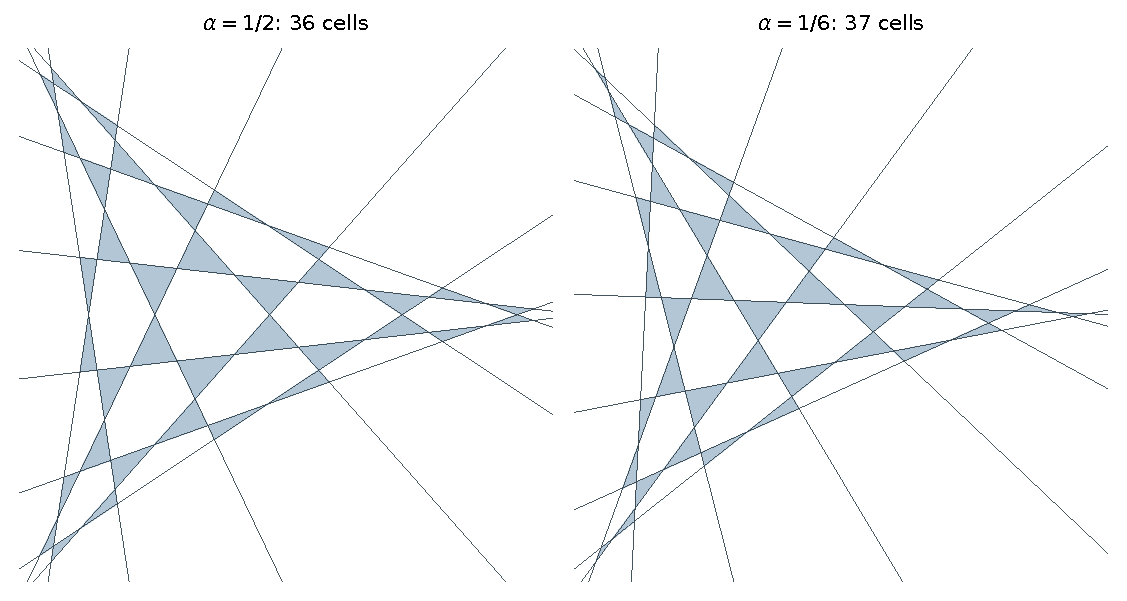
\includegraphics[width=0.9\linewidth]{phase-family.pdf}
\caption{New rational-coordinate illustrations at $n=12$, obtained from the half-phase and shifted trigonometric families. Two independent exact counters certify 36 and 37 triangles in these rational proxies. The axes of each panel are rescaled independently. The real-coordinate universal theorem follows from the symbolic sign and modular arguments, independently of this illustration. The underlying family is attributed to F\"uredi and Pal\'asti.}\label{fig:phase}
\end{figure}

\subsection{Projective changes of affine chart}

The shifted count is enough for the even part of~\eqref{eq:G}. To obtain the additional odd-order gain we use exposed vertices of the half-phase arrangement. The exact coordinate map is
\begin{equation}\label{eq:projective-map}
(x,y)\longmapsto \left(\frac{x}{h-x},\frac{y}{h-x}\right),\qquad h\ne0.
\end{equation}
It replaces the line $x=h$ by the line at infinity. The transformed coefficients of $ax+by=c$ are
\begin{equation}\label{eq:line-transform}
\Phi_h(a,b,c)=(ha-c,hb,c).
\end{equation}
Unlike an affine transformation, this change can alter which projective triangular faces appear bounded. Thus counting triangles before and after the change requires an explicit sign argument.

\begin{lemma}[Exact covariance]\label{lem:projective-covariance}
If $D(\ell,m)\ne0$, then
\begin{align}
D(\Phi_h\ell,\Phi_hm)&=hD(\ell,m)(h-x_{\ell m}),\\
E(\Phi_hr;\Phi_h\ell,\Phi_hm)&=h^2E(r;\ell,m),\\
O(\Phi_hr;\Phi_h\ell,\Phi_hm)&=h^3(h-x_{\ell m})O(r;\ell,m),\label{eq:projective-sign}
\end{align}
where $x_{\ell m}$ is the abscissa of the old intersection. If the cut avoids every old vertex, the transformed arrangement has no parallel pairs. Triple nonconcurrence is preserved.
\end{lemma}
\begin{proof}
Substitute~\eqref{eq:line-transform} into the polynomial expressions in Section~\ref{sec:geometry}, expand, and cancel. Nonzero $h$ and avoidance of all $x_{\ell m}$ give the pair determinant claim, while multiplication by $h^2$ preserves a nonzero triple evaluation.
\end{proof}

The sign multiplier in~\eqref{eq:projective-sign} also gives a direct triangle-preservation rule. If $h>0$ and all vertices of a certified triangle lie to the left of $x=h$, all three multipliers are positive. If $h<0$ and its vertices lie to the right, they are again positive. At selected exposed vertices on the opposite side, the sign reverses. Carefully choosing which vertices are separated by the cut creates the extra triangles.

\begin{lemma}[One exposed vertex]\label{lem:one-cap}
For odd $n=2m+1\ge3$, a change of affine chart of the half-phase arrangement has at least $\B(n)+1$ bounded triangles.
\end{lemma}
\begin{proof}
The intersection of $\ell(x)$ and $\ell(y)$ has abscissa
\begin{equation}\label{eq:vertex-x}
X(x,y)=\cos(2x)+\cos(2y)+\cos(2x+2y).
\end{equation}
For the half-phase angles, the vertex of lines $0,n-1$ is uniquely rightmost, with abscissa $c_n=1+2\cos(\pi/n)>0$. Indeed, each of the first two cosine terms in~\eqref{eq:vertex-x} is at most $\cos(\pi/n)$ and the last is at most one; if the pair is not $(0,n-1)$, at least one necessary inequality is strict. Choose $h>0$ between all other abscissae and $c_n$.

No selected triangle of~\eqref{eq:halfphase-triples} uses the pair $(0,n-1)$: such a triple would require its middle index to be $0$ or $n-1$ modulo $n$. Hence all counted triangles are preserved by the positive multiplier rule. The additional triple $(0,m,2m)$ has, for each test line, nonnegative evaluation at the exposed vertex and nonpositive evaluations at its other two vertices before the transformation. The cut reverses exactly the exposed-vertex sign, so the transformed triple satisfies the certificate. These signs follow from~\eqref{eq:trig-oriented} by splitting the test index at $m$. The triple is absent from the old selected list, and Lemma~\ref{lem:projective-covariance} preserves simplicity. This gives one additional bounded triangle.
\end{proof}

\begin{lemma}[Two exposed vertices]\label{lem:two-caps}
For $n=6k+3$ with $k\ge1$, a change of affine chart of the half-phase arrangement has at least $\B(n)+2$ bounded triangles.
\end{lemma}
\begin{proof}
Write $n=3m$, where $m=2k+1$. The two intersections supported by $(m-1,m)$ and $(2m-1,2m)$ have common abscissa $-c_n/2$. Every other intersection has strictly larger abscissa. To verify the latter assertion, rewrite~\eqref{eq:vertex-x} as
\[
X(u,v)=2zw+2z^2-1,
\qquad z=\cos(u+v),\quad w=\cos(u-v).
\]
For nonadjacent angle indices, the cosine bounds on the discrete grid, together with completing the square in $z$, give $X>-c_n/2$. For adjacent indices, $w=\cos(\pi/n)$ and the same quadratic attains equality precisely at $u+v=2\pi/3$ or $4\pi/3$, giving the two listed pairs. The exceptional wrapping pair $(0,n-1)$ is the rightmost vertex. These exposure inequalities are proved uniformly in \lean{FurediPalastiCaps.lean}.

Choose $h<0$ strictly above $-c_n/2$ and below all other abscissae. The modular conditions~\eqref{eq:halfphase-triples} show that no counted triangle uses either exposed pair. Its vertices are therefore all to the right of the cut and its signs are preserved. The two additional support triples are
\[
(2k,2k+1,5k+2),\qquad (k,4k+1,4k+2).
\]
For each test index, substitution into~\eqref{eq:trig-oriented} gives one sign at the exposed pair and its opposite weak sign at the other two vertices. The negative cut reverses exactly the exposed-vertex multiplier in each case, establishing the transformed certificates. The two triples are distinct and neither satisfies the old selection residues. Simplicity follows from Lemma~\ref{lem:projective-covariance}. Appending both triples to the retained list proves the claim.
\end{proof}

\begin{figure}[tbp]
\centering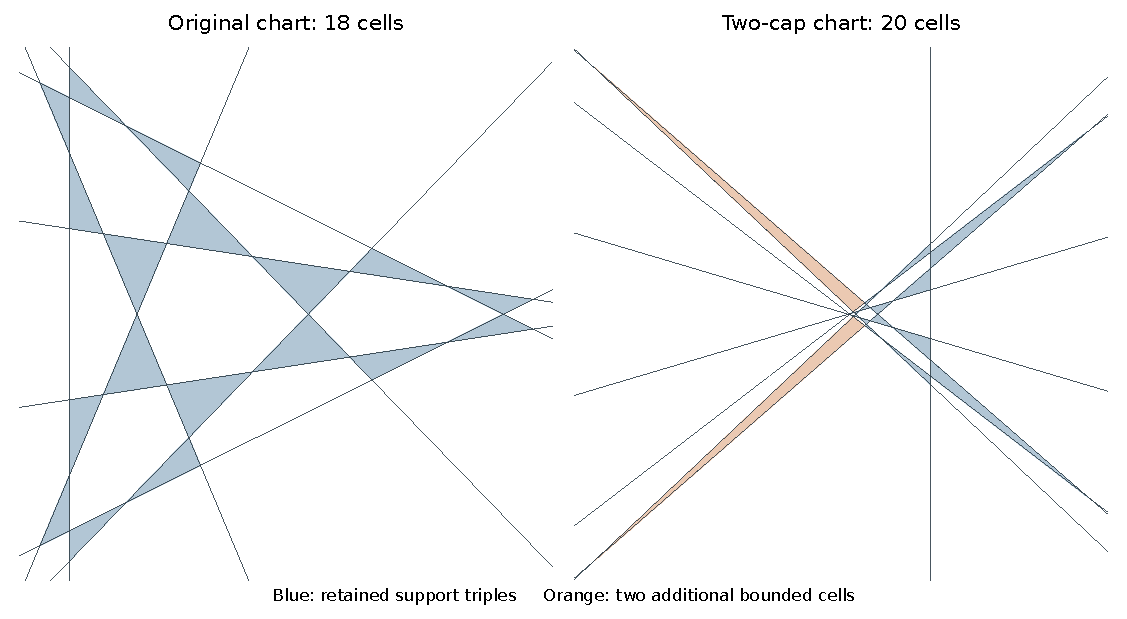
\includegraphics[width=0.95\linewidth]{affine-chart.pdf}
\caption{New exact rational illustration at $n=9$: the change of affine chart retains all 18 old triangular cells and creates two more. The resulting 20 is below the known optimum 21; this figure illustrates the uniform mechanism. Panels are rescaled independently. Both counts are checked exactly. The general proof tracks the determinant multiplier at every vertex, independently of the drawing.}\label{fig:chart}
\end{figure}

\subsection{Assembly, exact gain, and asymptotic scale}

\begin{proof}[Proof of Theorem~\ref{thm:main}]
Use Lemma~\ref{lem:shifted-count} for even $n\ge4$. For odd $n$ not divisible by three, $n(n-3)\equiv1\pmod3$, so
$\B(n)+1=\floor{n(n-3)/3}+2$; apply Lemma~\ref{lem:one-cap}. For odd multiples of three at least nine, $\B(n)=n(n-3)/3$ and Lemma~\ref{lem:two-caps} gives the same target. Three nonconcurrent lines give $\G(3)=1$, while the smaller cases have zero triangles. Each construction used is simple.
\end{proof}

\begin{corollary}[Exact improvement over the quoted baseline]\label{cor:gain}
For $n\ge4$,
\[
\G(n)-\B(n)=
\begin{cases}
1+(n\bmod2),&3\mid n,\\
n\bmod2,&3\nmid n.
\end{cases}
\]
The gains in classes $0,1,2,3,4,5\pmod6$ are respectively $1,1,0,2,0,1$.
\end{corollary}
\begin{proof}
The product $n(n-3)$ is zero modulo three when $3\mid n$, and one modulo three otherwise. Substitute these remainders in the floor and ceiling formulas.
\end{proof}

\begin{figure}[tbp]
\centering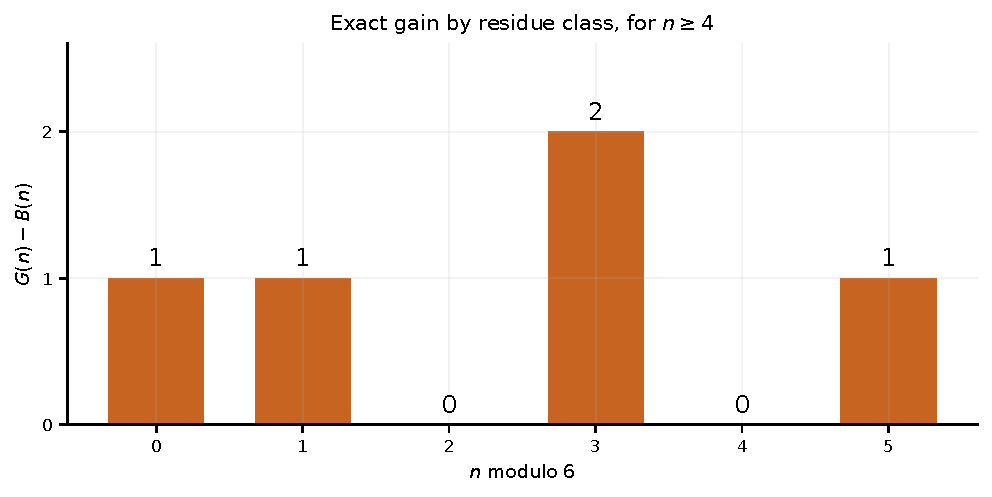
\includegraphics[width=0.88\linewidth]{residue-gains.pdf}
\caption{The exact proved gain $\G-\B$, resolved by residue class modulo six. The gain is strict on four classes; the universal statement includes arbitrarily large orders in each class.}\label{fig:residue}
\end{figure}

For comparison with the classical polynomial benchmark $\U(n)=\floor{n(n-2)/3}$, direct integer arithmetic gives, for $n\ge4$,
\begin{equation}\label{eq:gap}
\U(n)-\G(n)=\floor{\frac n3}+\mathbf1_{n\equiv2\ (3)}-1-(n\bmod2).
\end{equation}
This comparison does not formalize the published upper-bound theorem. It quantifies the scale of the remaining gap to that benchmark. It is still of order $n$, and stronger upper bounds or special constructions apply at some orders.

\begin{figure}[tbp]
\centering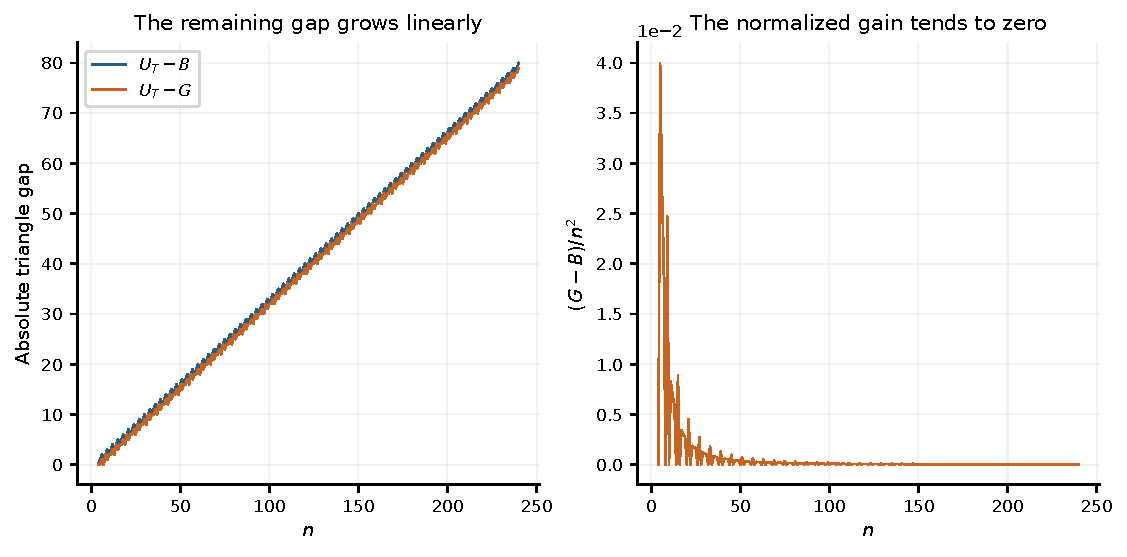
\includegraphics[width=0.94\linewidth]{normalized-gap.pdf}
\caption{Deficit and normalized growth computed from the proved formulas. The constant improvement is visible in the deficit, while both general lower formulas have the same leading quadratic and linear terms. The polynomial used in the deficit is a literature benchmark, not a new upper theorem of this paper.}\label{fig:normalized}
\end{figure}

The outcome is an unconditional affine theorem, stronger than the quoted baseline at infinitely many orders. Its numerical first priority remains a separate literature question. The construction gives a witness for each $n$; it does not provide an operation that adds one line to every preceding optimal witness.

\section{Individual cases, finite enhancements, and provenance}\label{sec:finite}

\subsection{The March values and their present verification}

The three finite inequalities associated with the author's early extension work are
\begin{equation}\label{eq:march-three}
\K(28)\ge238,\qquad \K(30)\ge275,\qquad \K(34)\ge357.
\end{equation}
Each now has an exact simple-arrangement certificate, so the same inequalities hold for $\Ks$. Their present validity is independent of the unproved recurrence in the original March manuscript. The certificates give actual lines and complete checked triangle lists, not only numerical consequences of an extension hypothesis.

The current OEIS table associates the name Zarzuelo with these entries~\cite{oeisA006066,zarzuelo2026}. Attribution in an index and first discovery are different questions. The earlier literature already contains matching constructions or consequences for some of these counts; the literature review records these overlaps. The claims made here are the documented attribution trail, the independently verified witnesses, and their place in the author's extension program. No new priority claim is inferred from the absence of a value from a particular online table.

\begin{figure}[tbp]
\centering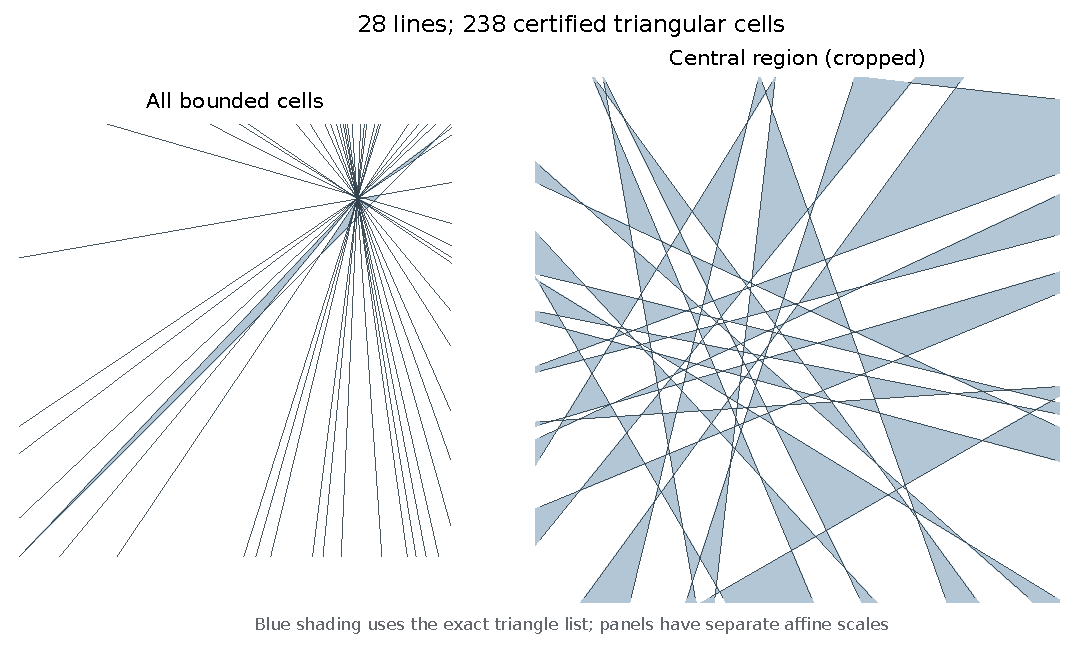
\includegraphics[width=0.96\linewidth]{historical-28.pdf}
\caption{The retained exact 28-line witness with 238 certified triangles. This is a new rendering of the saved coordinates associated with the earlier extension program. The marked zoom, where present, is an enlargement of the same arrangement; it does not add or remove lines from the certificate. The picture illustrates a lower bound, while the exact sign tests establish it.}\label{fig:historical28}
\end{figure}
\begin{figure}[tbp]
\centering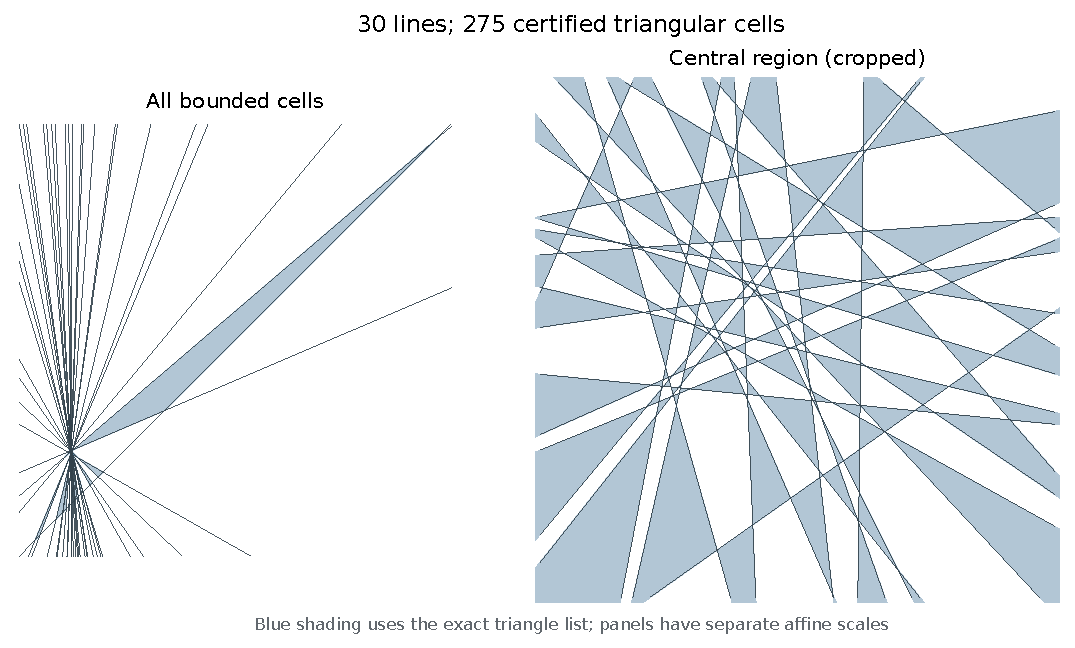
\includegraphics[width=0.96\linewidth]{historical-30.pdf}
\caption{The retained 30-line witness with 275 certified triangles, rendered from its exact coordinates. The count has prior literature overlap and is not asserted to be a new numerical record. The complete witness remains in the catalog even though the historical general extension proof was incomplete.}\label{fig:historical30}
\end{figure}
\begin{figure}[tbp]
\centering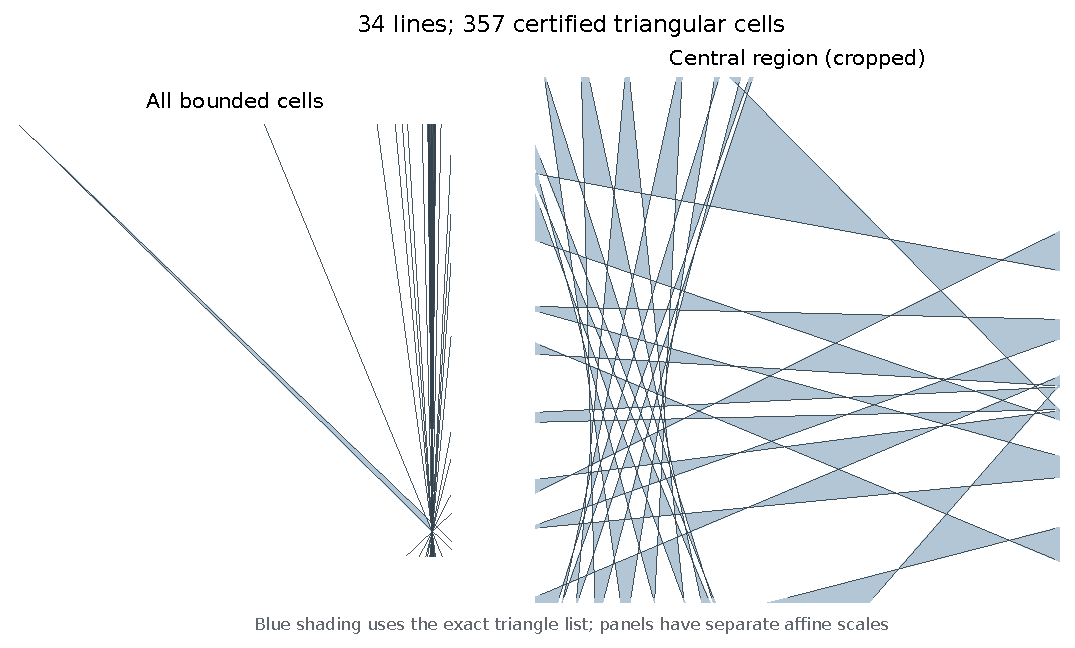
\includegraphics[width=0.96\linewidth]{historical-34.pdf}
\caption{The retained 34-line witness with 357 certified triangles. Original plotting of the certificate makes the finite conclusion inspectable independently of the claimed universal extension. The construction input and earlier matching literature are credited separately.}\label{fig:historical34}
\end{figure}

The original inventory also listed outputs for every order from 3 through 60, together with larger cases at 99 and 195. Some were direct certificates, some were numerical consequences of a boundary-defect argument, and many were weaker than an already available construction. Appendix~\ref{app:historical} preserves that inventory as history. The current certificate aliases independently retain its numerical inequalities; a label inherited from the old table is not used as a present formal-proof status.

\subsection{Materialized improvements from the phase and chart construction}

Table~\ref{tab:finite-refinement} records simple rational witnesses promoted during the last construction phase. Each listed new count is supplied by the universal theorem and also realized by an independently checked finite coordinate file. This double presentation is useful: the theorem proves all orders, while the coordinates support visualization and further exact searches.

\begin{table}[tbp]
\centering
\begin{tabular}{@{}rrrr@{}}
\toprule
$n$ & Earlier retained count & Current simple count & Increase\\
\midrule
39&469&470&1\\
47&690&691&1\\
48&720&721&1\\
51&817&818&1\\
53&884&885&1\\
54&918&919&1\\
55&954&955&1\\
59&1102&1103&1\\
60&1140&1141&1\\
99&3169&3170&1\\
195&12481&12482&1\\
\bottomrule
\end{tabular}
\caption{Changes relative to this project's previous retained witnesses, not a table of first discoveries or global record improvements. ``Simple'' is certified for every current coordinate witness in this table.}\label{tab:finite-refinement}
\end{table}

In particular, the earlier additional-line values $39:469$, $51:817$, $99:3169$ and $195:12481$ are now exceeded by $\G$ itself. Their finite correctness survives, but those numbers are not distinctive of the additional-line family. Historical evidence is retained rather than deleted when a stronger construction is found.

\subsection{The 44-line simple case}

The exact exterior extension of the retained 43-line arrangement creates 21 triangles while preserving its 587 old triangles. Both exact counters and the Lean certificate give a simple 44-line arrangement with 608 triangles. The published simple upper bound of Blanc at this order is also 608~\cite{blanc2011}. Thus, using that external upper theorem,
\begin{equation}\label{eq:44-simple}
\Ks(44)=608.
\end{equation}
The repository proves the lower inequality. It does not formally prove Blanc's theorem, and~\eqref{eq:44-simple} does not establish $\K(44)=608$ in the unrestricted classical problem. Nor does materializing this consequence establish first discovery of the numerical value.

This example shows why upper-bound scope belongs next to the numerical statement. A simple witness can establish a classical lower bound, but a simple upper theorem cannot by itself close the classical problem.

\subsection{External records and independently checked inputs}

The updated catalog incorporates exact gallery witnesses from Parpalak and Utkin at
\[
8:15,\ 14:54,\ 20:117,\ 26:204,\ 32:315,\ 36:402,\ 38:450,\ 42:553,\ 46:667,\ 50:792.
\]
These are constructions or coordinate sources of the cited researchers, not newly discovered values in this project. The eight-line value has older priority; the modern gallery is the source of the checked coordinates. The public source snapshot and the formal certificate index preserve the provenance~\cite{parpalakutkin2026,oeisA006066}.

All fifteen of Maiorana's supplied 14-line arrangements with 54 triangles were independently checked and promoted as finite certificates~\cite{maiorana2026}. Fourteen have two triple points and one has four. Their source license and immutable commit are retained. These witnesses are a particularly useful warning against conflating simple and nonsimple arrangements: removing a multiple intersection by a small perturbation need not preserve the full triangle count. Section~\ref{exp:section} reports the exact resolution experiments.

The two source snapshots used for these imports are Maiorana commit
\nolinkurl{e47c7cfd9661e54d29befb83118bf83d5f804028} and gallery commit
\nolinkurl{feae4f5571a988a3ed45bd26a36259ebb7d7d3d2}. Their mathematical attribution is attached to each source record even when a new Lean wrapper or new figure is generated here.

\subsection{The finite envelope and the complete tables}

\begin{proposition}[Retained all-order envelope]\label{prop:envelope}
Let $C(n)$ be the maximum count in the finite catalog at order $n$, or zero if that order is absent. Then $\K(n)\ge\Lbound(n)=\max\{\G(n),C(n)\}$ for every $n$. In the frozen release, $\Lbound(n)=\G(n)$ for every $n>195$.
\end{proposition}
\begin{proof}
When $C(n)\le\G(n)$, use Theorem~\ref{thm:main}. Otherwise choose a certificate attaining the finite maximum and apply Proposition~\ref{prop:finite-sound}. No coordinate certificate in this release has order greater than 195. Larger computational witnesses discussed later have not been silently added to the Lean catalog.
\end{proof}

The formal definition is \lean{Universal.bound = max Universal.baseline AllN.bound}. Since $\G\ge\B$, it equals the expression in Proposition~\ref{prop:envelope}; the older \lean{AllN} layer preserves the previous finite-envelope theorem. This makes comparisons reproducible without rewriting the historical construction history.

\begin{figure}[tbp]
\centering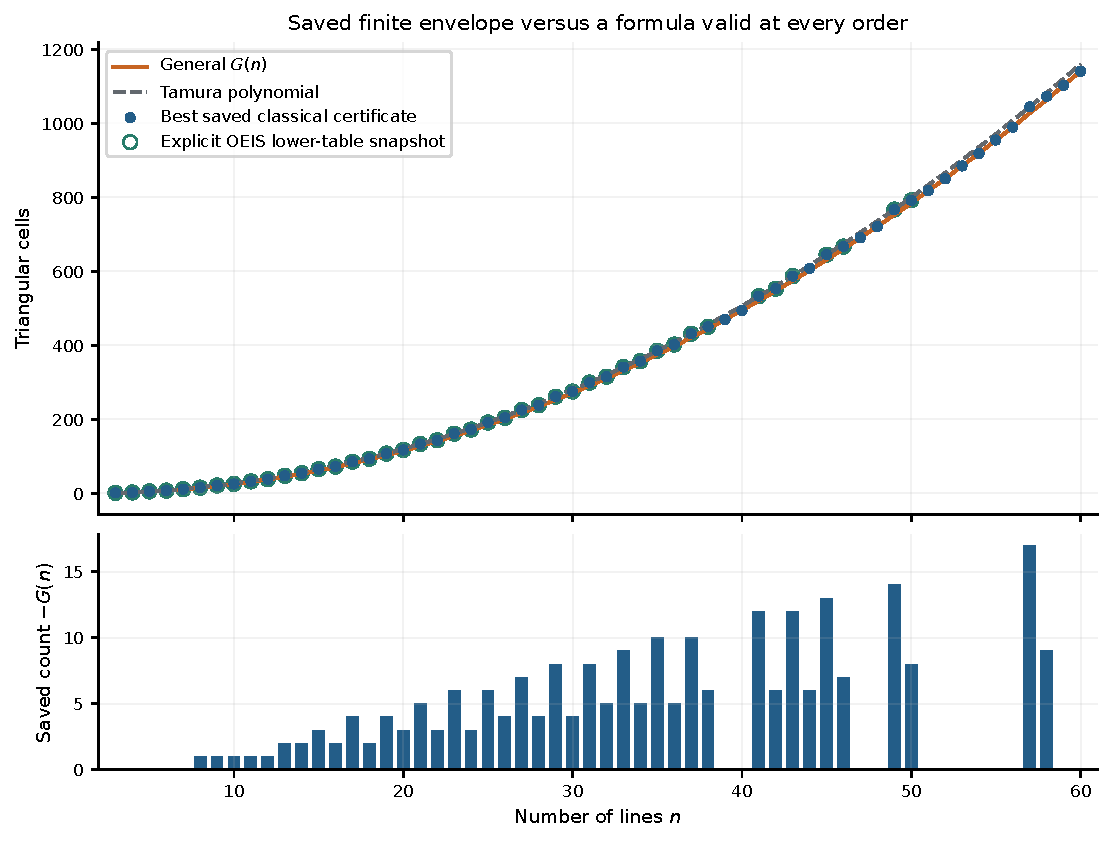
\includegraphics[width=0.96\linewidth]{finite-envelope.pdf}
\caption{The strongest saved simple and classical coordinate counts, compared with the uniform formula and the polynomial upper benchmark. External witnesses retain their attribution. A marker above $\G$ is a finite enhancement of the general formula, not automatically an original record.}\label{fig:finite-envelope}
\end{figure}

Appendix~\ref{app:finite-table} gives the best saved simple and classical values from 3 through 60. Appendix~\ref{app:catalog} lists all 138 certificate identities, including repeated orders and weaker checkpoints. Appendix~\ref{app:historical} gives the older author-output inventory. Together these tables prevent three common confusions: a retained output is not necessarily the best available value; a missing OEIS row is not proof of novelty; and an exact count for one arrangement is not automatically the extremal value $\K(n)$.

\section{Exterior extensions: the March proposal and its precise replacement}
\label{ext:section}

The starting point of this project was the March 2026 proposal that an odd
Kobon arrangement could always be extended with the gain
\begin{equation}
  \K(2m+2)\geq \K(2m+1)+m.
  \label{ext:march}
\end{equation}
The proposal was presented in \cite{zarzuelo2026} and subsequently described
as an iterative rule in \cite{handwiki2026}.  The preserved March source is
important evidence of the development of the idea, but is not a completed
proof of \eqref{ext:march}: its Lean file contains eight proof placeholders,
including the extension assertion.  The present work replaces the informal
alternating-segment argument by an actual geometric extension theorem and
identifies exactly which additional counting hypothesis yields the desired
gain.  Independently verified finite bounds are retained regardless of the
status of that original argument.

The later OEIS attribution at orders 28, 30, and 34 is evidence of the
proposal's reception, rather than a proof of numerical
priority~\cite{oeisA006066}.  In particular, the BBL table already records
the straight-line value $30:275$.  The perfect 33-line input belongs to
the family of Forge and Ram\'irez Alfons\'in~\cite{forge1998}; applying the
exterior extension stated by BBL gives $34:357$~\cite{bbl2008}.
The historical attribution, the validity of a finite count, and the
novelty of a general extension theorem are therefore assessed separately.

Two distinctions are essential.  A recurrence for maxima need not extend
\emph{every} arrangement attaining a given count, and a construction for one
odd-to-even step need not admit repeated full-gain extensions.  Throughout
this section the geometric hypotheses concern simple affine arrangements;
consequently their conclusions give lower bounds for both $\Ks$ and $\K$,
but nonsimple witnesses for $\K$ cannot automatically be substituted into
the hypotheses.

\subsection{A geometric theorem from explicitly visible pairs}

Write an old line as $L_i=\{p:\ell_i(p)=0\}$, with $\ell_i$ affine, and let
$A=\{L_0,\ldots,L_{n-1}\}$ be simple.  A linear functional $w$ is
\emph{admissible} if it is nonzero on every old line direction.  At
$p_{ij}=L_i\cap L_j$, choose the direction vectors $u_i,u_j$ on the two
supports so that $w(u_i)=w(u_j)=1$.  The following criterion uses only the
old arrangement.

\begin{definition}[Visible pair]
\label{ext:visible}
The pair $\{i,j\}$ is visible from $w$ if, for every old affine equation
$\ell_k$, the three real numbers
\[
  \ell_k(p_{ij}),\qquad D\ell_k(u_i),\qquad D\ell_k(u_j)
\]
have one common weak sign: either all are nonnegative or all are
nonpositive.  Here $D\ell_k$ denotes the linear part of $\ell_k$.
\end{definition}

Geometrically, the two increasing-$w$ rays bound an unbounded empty wedge.
The algebraic definition is convenient because it gives the required
half-plane inequalities directly, without assuming that a future triangle
already exists.

\begin{theorem}[Verified exterior realization]
\label{ext:realization}
Let $A$ be a simple arrangement of $n$ real affine lines, let $\mathcal T$
be a set of $T$ distinct triangular cells of $A$, and let $\mathcal V$ be
a set of $c$ distinct pairs visible from an admissible $w$.  If
\[
  H>\max_{i<j}w(p_{ij}),
\]
then adjoining $L=\{p:w(p)=H\}$ produces a simple arrangement containing
all triangles in $\mathcal T$ and at least $c$ further triangles.  In
particular, $\Ks(n+1)\geq T+c$.
\end{theorem}

\begin{proof}
Admissibility excludes a parallel old line, and the strict height
inequality excludes every old vertex from $L$.  Thus simplicity is
preserved.  Every old triangle lies in the convex hull of its vertices,
strictly below the level $H$, and survives unchanged.

For a visible pair, the new vertices on its two supports are
\[
 p_{ij}+(H-w(p_{ij}))u_i,
 \qquad p_{ij}+(H-w(p_{ij}))u_j.
\]
At either vertex an old affine equation has the form
\[
 \ell_k(p_{ij})+(H-w(p_{ij}))D\ell_k(u).
\]
The second coefficient is positive.  Definition~\ref{ext:visible}
therefore puts all three vertices in one closed half-plane of each old
line.  The new line is itself a supporting side, and the triangle is
nondegenerate because the old intersection lies strictly below it.  No
arrangement line cuts its interior.  Different old pairs give different
support triples, and every new triple uses $L$, whereas no old one does.
The two lists are consequently disjoint.
\end{proof}

This is the geometric content of \texttt{Exterior.extension}.  The theorem
is proved for arbitrary real coefficients and either parity, with no
assumption about a future triangle count.  An explicit formal height is
\[
  H=1+\sum_{\substack{i,j<n\\i\ne j}}|w(p_{ij})|,
\]
so existence of a sufficiently distant line is part of the construction.
The proof uses the standard Lean logical axioms and no finite native
evaluation.  What it does \emph{not} supply is a universal lower bound of
$\lfloor n/2\rfloor$ on the number of visible pairs.

\subsection{Defect, boundary wedges, and a rule for both parities}

Let $t(A)=T$ and define the bounded-segment defect
\begin{equation}
 d(A)=n(n-2)-3T.
 \label{ext:defect}
\end{equation}
There are $n(n-2)$ elementary bounded segments.  A segment can support at
most one triangular cell: its endpoints determine the two other supports,
and their intersection lies on at most one side of the segment.  Thus
$d(A)$ counts the unused bounded segments.  Let $b(A)$ count the unbounded
two-sided cells, called wedges below.

\begin{lemma}[Boundary charging]
\label{ext:charging}
For a simple arrangement of $n\geq3$ lines,
\[
  3\leq b(A)\leq n,\qquad b(A)+d(A)\geq n.
\]
\end{lemma}

\begin{proof}
The arrangement has $2n$ free rays.  A wedge pairs two such rays at their
common endpoint, and each free ray belongs to at most one wedge.  An
unpaired ray on $L$, ending at $p=L\cap M$, meets an interior vertex of
$M$.  The two bounded elementary segments of $M$ incident to $p$ cannot
both support triangles: both triangles would also use the unique bounded
segment of $L$ starting at $p$.  Charge the unpaired ray to an unused
segment of $M$ at $p$.  Each unused segment receives at most two charges,
one at each endpoint.  Hence $2n-2b\leq2d$.  This also proves $b\leq n$.
Finally, the convex hull of all finite vertices has at least three
vertices.  Both supports at a hull vertex have free outgoing rays, which
give a wedge.  Distinct hull vertices give distinct wedges.
\end{proof}

Order the $2n$ oriented line directions cyclically.  The two directions
of a wedge are consecutive: a line direction strictly inside that sector
would force a line to enter the wedge and cross a free boundary ray.
Write $B\subset\mathbb Z/(2n)$ for the wedge-start indices.  Define
\begin{equation}
 c_j=\bigl|B\cap\{j,j+1,\ldots,j+n-2\}\bigr|,
 \qquad C(A)=\max_j c_j.
 \label{ext:profile}
\end{equation}
The $n$ directions on which an admissible $w$ is positive form one
consecutive block, and every such block occurs for some normal sector.
An exterior line closes precisely the wedges whose two rays lie in this
block.  Consequently $C(A)$ is the exact largest exterior gain and
\begin{equation}
 \sum_{j=0}^{2n-1}c_j=(n-1)b(A),\qquad
 \left\lceil\frac{(n-1)b(A)}{2n}\right\rceil
 \leq C(A)\leq\left\lfloor\frac n2\right\rfloor.
 \label{ext:average}
\end{equation}
The sum follows by counting the $n-1$ blocks containing a fixed wedge.
The upper bound follows because complete wedge pairs use disjoint rays
in a block of $n$ rays.

\begin{theorem}[Boundary-defect extension]
\label{ext:defect-theorem}
For a simple $n$-line arrangement with $n\geq3$ and $T$ triangles, an
exterior line preserves the old triangles and gives at least
\begin{equation}
 T+g(n,T),\qquad
 g(n,T)=\left\lceil\frac{n-1}{2n}
       \max\{3,\,3T-n(n-3)\}\right\rceil
 \label{ext:g}
\end{equation}
triangles.  Thus, for either parity,
\[
 \Ks(n)\geq T\quad\Longrightarrow\quad
 \Ks(n+1)\geq T+g(n,T).
\]
\end{theorem}

\begin{proof}
Lemma~\ref{ext:charging} gives
$b(A)\geq\max\{3,n-d(A)\}$.  Substitute into
\eqref{ext:average} and apply Theorem~\ref{ext:realization}.  If $T$ is
only a lower bound, the witness has some count $T'\geq T$; the right side
of \eqref{ext:g} is nondecreasing in $T$, which gives the stated
maximum-function implication.
\end{proof}

\begin{remark}[Formal scope and attribution]
\label{ext:defect-scope}
Theorem~\ref{ext:defect-theorem} is an ordinary geometric theorem in this
manuscript.  The cyclic sum, averaging argument, and defect arithmetic are
Lean checked, and Theorem~\ref{ext:realization} supplies actual geometric
realization.  The universal charging map and the correspondence between
Euclidean boundary rays and the finite cyclic data have not yet been
joined into an end-to-end Lean proof.  Exterior addition and
unused-segment arguments have precedents in
\cite{bbl2008,blanc2011}.  The contribution under investigation is the
explicit quantitative defect formulation and its certificate interface;
first numerical or historical priority is not asserted.
\end{remark}

\begin{corollary}[Full gain for an odd saturated input]
\label{ext:odd-full}
If a simple arrangement of $2m+1$ lines has defect at most two, an exterior
line creates exactly $m$ additional triangles.  In particular, this
applies to every simple odd arrangement attaining
$\lfloor n(n-2)/3\rfloor$.
\end{corollary}

\begin{proof}
The wedge count is at least $2m-1$.  If all $4m+2$ direction sectors had
gain at most $m-1$, then
\[
 2m(2m-1)\leq 2m b(A)=\sum_jc_j
 \leq(4m+2)(m-1)=2m(2m-1)-2,
\]
a contradiction.  Equation~\eqref{ext:average} bounds the gain above by
$m$.  The segment-count upper bound at odd $n$ leaves defect zero or two.
\end{proof}

For an even input $n=2m$, the sufficient condition $b(A)\geq2m-1$ likewise
forces gain $m$, because $(2m-1)^2>4m(m-1)$.  In either parity the exact
criterion is the finite condition $C(A)=\lfloor n/2\rfloor$.
There is no claim that every even or odd maximum has this boundary
profile.  Iterating \eqref{ext:g} is nevertheless legitimate ordinary
geometry and supplies a weaker lower-bound rule from any simple seed.

\subsection{What fails in indefinite full-gain exterior iteration}

The March argument made the number of new triangles follow from an
alternation assertion after placing a line far from all old vertices.
Distance proves preservation; it does not prove emptiness for half the
new segments.  For example, the five lines $y=ix+i^2$, $i=0,\ldots,4$,
have three triangles, and adding $y=x/2+100$ creates only one further
triangle.  These counts are checked by exact certificates.  This refutes
that unqualified step of the argument, without refuting a better choice
of line or an inequality about maxima.

A stronger obstruction concerns every chain of exterior additions.
Write $b_r$ for its wedge count and $c_r$ for the gain at step $r$.
Closing $c_r$ wedges consumes those wedges.  No new free ray can appear
at an old vertex, and a wedge at a new vertex must use one of the two
free rays of the newly added line.  Therefore
\begin{equation}
 b_{r+1}+c_r\leq b_r+2,
 \qquad
 \sum_{j<r}c_j\leq b_0+2r-b_r\leq b_0+2r-3.
 \label{ext:budget}
\end{equation}
The accumulated exterior gain is at most linear in the number of steps.
The accumulated gains $\lfloor n/2\rfloor$ are quadratic, so an infinite
chain of such full-gain exterior steps is impossible.  The numerical
contradiction is formalized in
\texttt{Iteration.no\_infinite\_full\_gain\_budget}; as in
Remark~\ref{ext:defect-scope}, the universal wedge-budget interpretation
is an ordinary geometric argument.

\begin{table}[tb]
\centering
\small
\begin{tabular}{rrrrr}
\hline
Input order & Triangles & Wedges & Best exterior gain & Requested gain\\
\hline
49&767&47&24&24\\
50&791&24&23&25\\
51&814&3&2&25\\
52&816&3&2&26\\
53&818&3&2&26\\
\hline
\end{tabular}
\caption{One exact greedy exterior chain from the attributed 49-line
input.  Every direction sector was counted with rational arithmetic.
These are capacities of the displayed arrangements, not upper bounds
for $\K$ or $\Ks$ at the corresponding orders.}
\label{ext:49-table}
\end{table}

Table~\ref{ext:49-table} records the motivating test from $49:767$.
The obstruction is independent of the greedy tie break: two exterior
gains $24$ and $25$ from this seed would imply
\[
 b_2\leq47+4-24-25=2,
\]
contrary to $b_2\geq3$.  The five finite profile maxima have a checked
Lean arithmetic certificate; their identification with the saved
coordinates is supplied by the exact geometry program.  A reconstruction
between steps or an interior insertion could evade this boundary budget,
so it does not disprove the proposed recurrence for maxima.

\begin{figure}[tb]
\centering
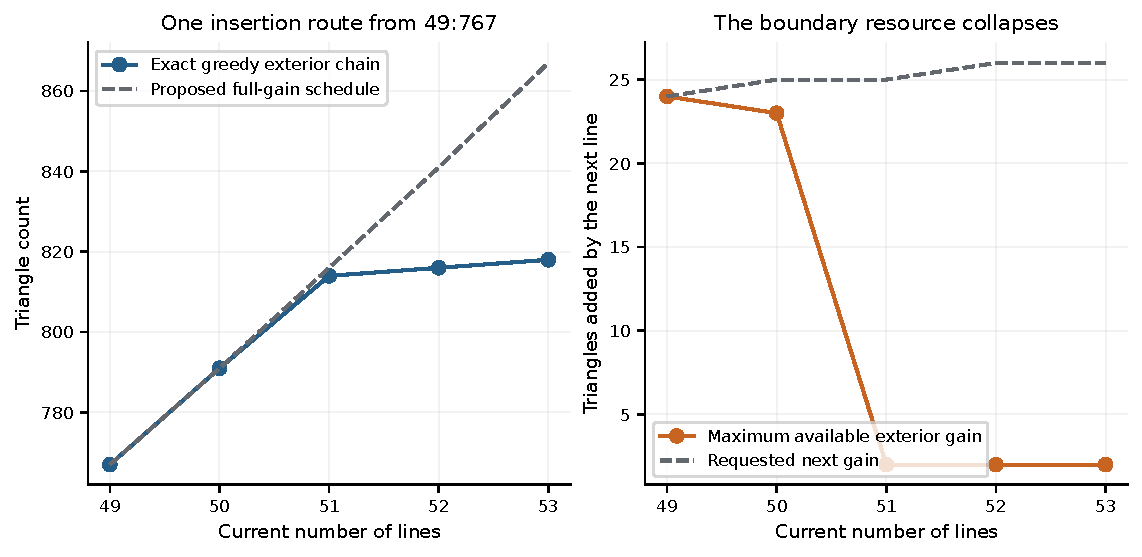
\includegraphics[width=0.88\linewidth]{figures/successor-49-resource.pdf}
\caption{The boundary resource in the particular exact 49-line chain.
The sharp drop in available wedges explains why its first full-gain
extension cannot be repeated with the requested next gain.  The plotted
capacities concern this chain only.}
\label{fig:successor}
\end{figure}

\subsection{A conditional recurrence and an unconditional numerical bound}

For any integer-valued function $F$, assume
\begin{equation}
 F(n+1)\geq F(n)+\lfloor n/2\rfloor\qquad(n\geq s).
 \label{ext:full-step}
\end{equation}
Summation, including both parity cases, gives the fully checked arithmetic
implication
\begin{equation}
 F(n)\geq F(s)+
 \left\lfloor\frac{(n-1)^2}{4}\right\rfloor-
 \left\lfloor\frac{(s-1)^2}{4}\right\rfloor
 \qquad(n\geq s).
 \label{ext:conditional-closed}
\end{equation}
The hypothesis \eqref{ext:full-step} remains explicit in the formal
theorem.  Substituting $s=49$ and $F(49)=767$ yields the numerical target
\begin{equation}
 Q_{49}(n)=\left\lfloor\frac{(n-1)^2}{4}\right\rfloor+191.
 \label{ext:49-target}
\end{equation}

There is now a separate unconditional Lean theorem
\begin{equation}
 \K(n)\geq Q_{49}(n)\qquad(n\geq49),
 \label{ext:49-unconditional}
\end{equation}
proved using the saved witnesses at 49 and 50 and the classical all-order
baseline thereafter.  Indeed, for $n\geq51$,
\[
 \frac{n(n-3)}3-\frac{(n-1)^2}4-191
 =\frac{n^2-6n-2295}{12}\geq0,
\]
with equality at $n=51$ and an increasing numerator beyond it.  Rounding
gives $\B(n)\geq Q_{49}(n)$.  This proves the desired numerical formula
without constructing a nested full-gain chain.  The stronger all-order
bound $\G$ and the finite envelope elsewhere in this paper also dominate
it.

For comparison, direct iteration of the defect rule
$T_{n+1}=T_n+g(n,T_n)$ from $49:767$ guarantees
$50:791$, $51:803$, $52:805$, and $60:821$.
The stronger target \eqref{ext:49-target} gives $51:816$, $52:841$, and
$60:1061$.  These are different constructions and different assertions.
The completed numerical theorem does not retrospectively prove the
March extension claim, and the failure of its proposed exterior
iteration does not invalidate the completed numerical theorem.

\section{Compatible seeds, geometric doubling, and sparse families}
\label{fam:section}

The second extension mechanism inserts a whole collection of lines near
a distinguished support.  It belongs to Bartholdi, Blanc, and Loisel
(BBL)~\cite{bbl2008}; it is fundamentally different from the one-line
exterior operation of Section~\ref{ext:section}.  The present work supplies
explicit compatible seeds, an actual one-step geometric Lean proof, and
finite certificates at considerably larger orders.  The distinction
between a published-theorem consequence and a completed recursive Lean
theorem is maintained throughout.

\subsection{The exact one-step theorem}

Let $q=4r$ with $r\geq5$, put $\alpha=\pi/q$, and take
\begin{equation}
  0<\varepsilon<\tan(\alpha/2).
  \label{fam:epsilon}
\end{equation}
Define $q$ ordered intercepts, indexed from zero, by
\begin{equation}
 a_j=
 \begin{cases}
 \tan((j-q/2+1)\alpha),&0\leq j<q/2-1,\\
 -\varepsilon,&j=q/2-1,\\
 \varepsilon,&j=q/2,\\
 \tan((j-q/2)\alpha),&q/2<j<q.
 \end{cases}
 \label{fam:old-grid}
\end{equation}
In particular, the extreme intercepts are $-\cot\alpha$ and
$\cot\alpha$.  The two central intercepts replace the repeated zero that
would otherwise occur in this grid.

\begin{definition}[Compatible tangent-grid seed]
\label{fam:compatible}
A seed at $(q,\varepsilon)$ consists of $Y_0:y=0$ and the $q$ lines
$L_j:y=m_j(x-a_j)$, with the following properties: the arrangement is
simple; every interval $[a_j,a_{j+1}]$ on $Y_0$ supports the triangular
cell with supports $Y_0,L_j,L_{j+1}$; and the central apex
$L_{q/2-1}\cap L_{q/2}$ lies above $Y_0$.  A counted seed additionally
carries a list of distinct actual triangular cells whose length is at
least $T$.
\end{definition}

Simplicity already requires all $m_j$ to be nonzero and pairwise distinct.
The distinguished-line condition is a substantial geometric restriction,
not a consequence of having a large total count.  It is precisely why
an arbitrary optimal arrangement cannot simply be used as a repeatable
BBL seed.

\begin{theorem}[Fully verified geometric doubling]
\label{fam:doubling}
Suppose $q=4r\geq20$ and \eqref{fam:epsilon} holds.  A compatible
tangent-grid seed with at least $T$ certified triangles gives a simple
real straight-line arrangement of $2q+1$ lines with at least
\begin{equation}
  T+q^2
  \label{fam:gain}
\end{equation}
triangles.
\end{theorem}

The precise formal theorem is \texttt{BBLDoubling.doubling}.  It assumes
the actual old line equations, simplicity, each distinguished triangle,
the positive central height, and a duplicate-free triangle list.  It
does not assume a future crossing order, a list of future empty
triangles, or a triangle-count recurrence.  Its conclusion is an actual
\texttt{SimpleLowerBound}; the generic proof uses only the standard Lean
logical axioms.  The numerical doubling principle is BBL's.  The
contribution here is its completed geometric proof for these explicit
hypotheses, using the following two-parameter realization.

\begin{proof}[Geometric proof and its formal decomposition]
For $0\leq i<q$ set
\[
 \beta_i=-\frac\pi2+(i+\tfrac12)\alpha,
 \qquad b_i=\tan\beta_i.
\]
Adjoin the lines
\begin{equation}
 M_i:\quad y=\kappa g_i(\delta)(x-b_i),\qquad
 g_i(\delta)=\frac{2b_i}{1+b_i^2}+\frac\delta{b_i}
            =\sin(2\beta_i)+\delta\cot\beta_i.
 \label{fam:pencil}
\end{equation}
Choose $\delta>0$ sufficiently small and then $\kappa>0$ sufficiently
small relative to the fixed $\delta$ and the seed.  This order of choices
is part of the proof.  BBL's published construction uses explicit scales;
the qualitative two-scale statement here is established independently
by the formal crossing analysis, rather than inferred from those fixed
scales.

For two new lines put $t=b_i$ and $u=b_k$.  Their intersection has
$x$-coordinate independent of $\kappa$:
\begin{equation}
 X_{ik}(\delta)=
 \frac{2tu(t+u)}{2tu(1-tu)-\delta(1+t^2)(1+u^2)}.
 \label{fam:crossing}
\end{equation}
When $tu\ne1$, its limit is the reduced tangent
$(t+u)/(1-tu)=\tan(\beta_i+\beta_k)$, and the exact displacement is
\begin{equation}
 X_{ik}(\delta)-\frac{t+u}{1-tu}
 =\frac{\delta(t+u)(1+t^2)(1+u^2)}
 {[2tu(1-tu)-\delta(1+t^2)(1+u^2)](1-tu)}.
 \label{fam:displacement}
\end{equation}
For sufficiently small positive $\delta$ its nonzero sign is that of
$(t+u)tu$.  If $tu=1$, the crossing diverges along the specified exterior
ray as $\delta\downarrow0$; if $t+u=0$, its coordinate is exactly zero.
Thus neither exceptional case is hidden inside a continuity argument
with a vanishing denominator.

The reduced tangents, the old intercepts, the new half-grid intercepts,
and $-\varepsilon,0,\varepsilon$ determine a strictly ordered finite
system of cuts.  Equations~\eqref{fam:crossing}--\eqref{fam:displacement}
place every new--new crossing in its prescribed cut interval.  Taking
$\delta$ in the intersection of the finitely many resulting positive
neighborhoods also makes the new slope factors nonzero and distinct.
For fixed such $\delta$, each old--new intersection tends to the
corresponding old intercept as $\kappa\to0$.  Finite continuity then
realizes all the prescribed strict crossing comparisons simultaneously.
Small $\kappa$ separates old and new slopes.  Injectivity along each new
crossing row excludes new triple intersections; old simplicity excludes
the remaining ones.  This proves actual simplicity and crossing order.

The count can now be separated from trigonometry.  Treat the $q$ new lines
and $Y_0$ as $q+1$ auxiliary supports.  The integer row model places old
support $j$ at key $4j+2$.  A pair of auxiliary supports with crossing key
$z$ yields a mixed triangle with old support $j$ when
\begin{equation}
  |z-(4j+2)|<4.
  \label{fam:neighbors}
\end{equation}
Every auxiliary pair has two such old neighbors, except for at most $q$
exterior pairs, each of which has one.  Hence the number is at least
\begin{equation}
 2\binom{q+1}{2}-q=q^2.
 \label{fam:mixed-count}
\end{equation}
The row inequalities make two sides consecutive on their supports.
The two-side emptiness lemma proves that the corresponding triangle is
an actual empty cell.  The supporting triples are distinct.  Thus
\eqref{fam:mixed-count} counts genuine triangles, not merely local
crossing patterns.

It remains to preserve the seed's contribution.  An old triangle not
using $Y_0$ has a strict half-plane sign against $Y_0$; all new lines
converge to $Y_0$, so its three vertex signs persist for sufficiently
small $\kappa$.  The old triangles with a side on $Y_0$ require a different
argument.  Saturation forces consecutive old apices to have opposite
heights.  The positive central apex fixes the alternating parity.
The crossing order identifies a new cap support for each noncentral
distinguished triangle.  On both cap endpoints, every new line has the
parity-correct weak sign; strict signs against other old supports
persist by continuity.  This replaces each such old triangle by one
empty triangle with the same two old supports.  The central triangle
itself is retained.  The finite cap and noncap requirements can again
be satisfied by one common positive $\kappa$.

Finally, these $T$ retained or replaced triangles have at least two old
nonhorizontal supports, while the $q^2$ mixed triangles have two
auxiliary supports.  The supporting triples cannot coincide.  Their
union is a duplicate-free witness of length at least $T+q^2$.
\end{proof}

The recurrence preserves the certified segment deficit:
\begin{equation}
 \Delta(q,T)=q^2-1-3T,\qquad
 \Delta(2q,T+q^2)=\Delta(q,T).
 \label{fam:deficit-preserved}
\end{equation}
Here the equality concerns the transported lower count; if the output
has additional uncounted triangles, its actual defect can be smaller.
Thus doubling amplifies a compatible seed to larger orders while
preserving its certified constant deficit.  A smaller-defect seed or a
new source of additional triangles is needed to improve that deficit.

\subsection{The compatible eleven-line realization}

The useful eleven-line count is $32$, an existing result; the search
started from the Honma-based construction displayed by
Savchuk~\cite{savchuk2025}.  The additional work here is an explicit
realization compatible with the BBL grid for arbitrarily small positive
central separation.  Take $Y_0:y=0$ and
\begin{equation}
 x-v_jy=a_j,\qquad
 (v_0,\ldots,v_9)=\tfrac1{10}(15,-2,14,1,4,-4,5,-3,12,-5),
 \label{fam:seed11-slopes}
\end{equation}
where
\begin{equation}
 (a_0,\ldots,a_9)=
 (-\tan\tfrac{4\pi}{10},-\tan\tfrac{3\pi}{10},
 -\tan\tfrac{2\pi}{10},-\tan\tfrac{\pi}{10},
 -\varepsilon,\varepsilon,
 \tan\tfrac{\pi}{10},\tan\tfrac{2\pi}{10},
 \tan\tfrac{3\pi}{10},\tan\tfrac{4\pi}{10}).
 \label{fam:seed11-grid}
\end{equation}
For every $0<\varepsilon\leq10^{-5}$ the seed is simple, has at least
32 certified triangles, and has all nine distinguished triangles.
Its central slopes are $5/2$ and $-5/2$ and its central height is
$5\varepsilon/2>0$.

The stability check is finite but uniform in $\varepsilon$.  The
determinant for a triple of nonhorizontal lines is affine in the
intercepts and therefore affine in $\varepsilon$:
\[
 D_{ijk}=(a_j-a_k)v_i+(a_k-a_i)v_j+(a_i-a_j)v_k.
\]
Exact rational enclosures for the four tangent values and endpoint
sign checks certify the whole interval.  The first certificate used
outward rational interval arithmetic; the subsequent Lean theorem uses
proved trigonometric enclosures and the parametric certificate soundness
theorem.  The limit $\varepsilon=0$ is used only to bound expressions;
it is not presented as a simple arrangement.  Five visible pairs for
$w=(10,-13)$ are also proved uniformly, giving the actual exterior bound
$12:37$ by Theorem~\ref{ext:realization}.

\begin{figure}[tb]
\centering
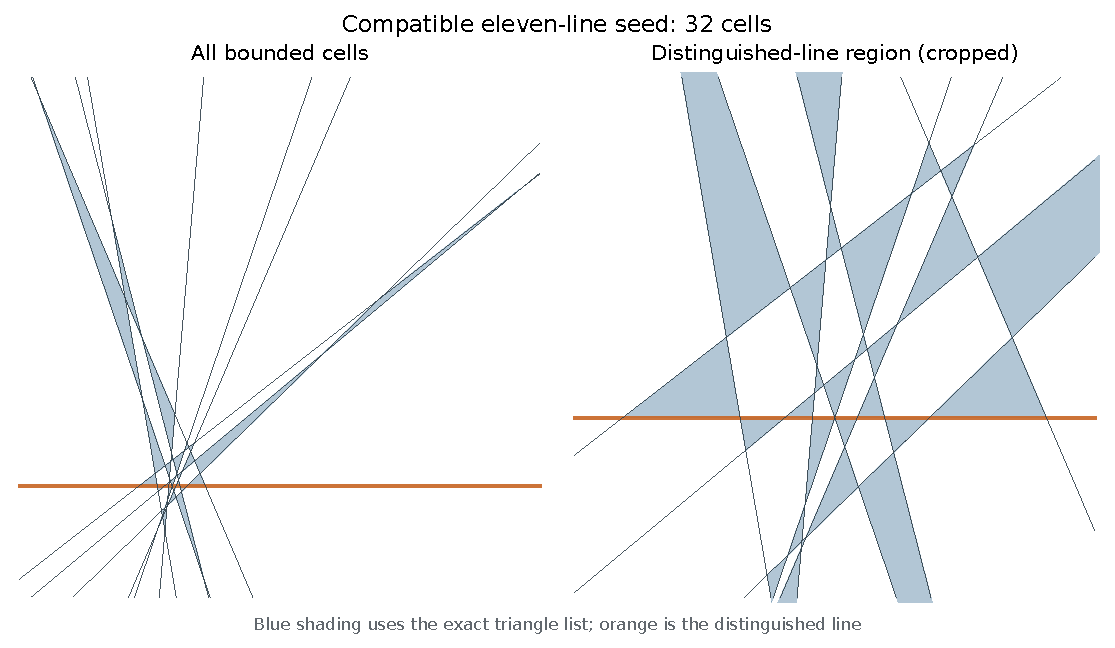
\includegraphics[width=0.88\linewidth]{figures/seed-11.pdf}
\caption{A finite rational realization of the compatible eleven-line
seed, with global and distinguished-line views.  The figure illustrates
the arrangement; the all-small-parameter
claim is certified by exact determinant and half-plane inequalities,
not by the rendering.  The count $32$ is inherited from earlier work;
the compatible realization and parameter certificate are the contribution
recorded here.}
\label{fig:seed11}
\end{figure}

Using the published BBL construction, with its finite-depth choice of
the exceptional parameter, gives the ordinary mathematical family
\begin{equation}
 q_t=10\cdot2^t,\qquad N_t=q_t+1,\qquad
 \Ks(N_t)\geq T_t=\frac{100\cdot4^t-4}{3}.
 \label{fam:eleven-family}
\end{equation}
The arithmetic is
\[
 T_0=32,\quad T_{t+1}=T_t+q_t^2,
 \quad
 T_t=32+100\sum_{j<t}4^j=\frac{q_t^2-4}{3}.
\]
The BBL geometric theorem and its iteration mechanism retain their
original attribution.  The formula is one below
$\lfloor N_t(N_t-2)/3\rfloor=(q_t^2-1)/3$; at $N_0=11$ the sharper known
upper bound is already $32$~\cite{savchuk2025}.
The checkpoints $21:132$ and $41:532$ are weaker than the known
$21:133$ and $41:533$.  Thus the formula is not a record assertion at
every member.

The quantifiers matter.  For any prescribed finite depth $t$, one can
choose the starting exceptional parameter small enough for every step
up to $t$; the recorded application uses
$0<\varepsilon\leq\min\{10^{-5},(40\cdot2^t)^{-1}\}$.
A single fixed positive $\varepsilon$ working through infinitely many
steps is neither required nor claimed.  Equation~\eqref{fam:eleven-family}
is supported by the verified seed and the published BBL theorem.  It is
not yet an end-to-end infinite-family theorem in the Lean library:
Theorem~\ref{fam:doubling} starts at $q\geq20$, and its recursive witness
interface remains to be assembled as described below.

\subsection{Even companions and the stronger boundary invariant}

The arrangement in \eqref{fam:eleven-family} has defect three.  Theorem
\ref{ext:defect-theorem} therefore gives the paper-level infinite bound
\begin{equation}
 \Ks(q+2)\geq\frac{q^2-4}{3}+\frac q2-1,
 \qquad q=10\cdot2^t.
 \label{fam:even-defect}
\end{equation}
Indeed,
$g(q+1,(q^2-4)/3)=\lceil q(q-2)/(2(q+1))\rceil=q/2-1$.
The stronger value observed in all completed finite examples is
\begin{equation}
 \frac{q^2-4}{3}+\frac q2.
 \label{fam:even-strong}
\end{equation}
For $M=q+2$, equations~\eqref{fam:even-defect} and
\eqref{fam:even-strong} equal respectively
$M(M-5/2)/3-2$ and $M(M-5/2)/3-1$.
The polynomial is the relevant Blanc upper bound for \emph{simple}
arrangements in these residue classes~\cite{blanc2011}; it is not an
upper bound asserted here for unrestricted $\K(M)$, and small orders
can have sharper bounds.

\begin{proposition}[Conditional full-gain even family]
\label{fam:even-conditional}
If the compatible odd family admits at least $q/2$ visible pairs from
an admissible normal at each stage, then
\[
 \Ks(q+2)\geq\frac{q^2-4}{3}+\frac q2
 \qquad(q=10\cdot2^t).
\]
\end{proposition}

\begin{proof}
Apply Theorem~\ref{ext:realization} at each specified odd order.
\end{proof}

The working boundary argument supplies a concrete route to the premise,
rather than treating it as an unexplained numerical assumption.  Keep
$w=(10,-13)$ and require the rightmost old intercept line $R$ to have
slope $0<m_R<10/13$, with its rightmost vertex on $Y_0$.  Old visible
pairs avoiding $Y_0$ persist under a sufficiently small pencil, and at
most one visible old pair uses $Y_0$.  For $q=4r$ the proposed new pairs
are $r$ negative complementary pairs, $r-1$ positive almost-complementary
pairs, the pair formed by $Y_0$ and the rightmost new support, and a pair
formed by $R$ and the new support at
$\beta_* =\pi/4-\alpha/2$.  Their total is $q/2+1$, giving a net gain
of at least $q/2$ visible pairs after losing at most one.

The delicate last pair is governed by the strict maximum
\[
 \cot\alpha\sin(2\beta)+\cos(2\beta)-1
 =\frac{\sin(2\beta+\alpha)}{\sin\alpha}-1.
\]
On the half-grid it is uniquely maximal at $\beta_*$, with gap at least
$2\sin\alpha$ from every other index.  Its persistence under the
$\delta$ perturbation and then the scale ratio $\kappa/m_R$ is proved
for actual intersections.  The remaining assembly must compare this
maximum with all old vertices, transfer the $x$-order to $w$-order, and
preserve the rightmost-line hypothesis under reindexing.  A detailed
ordinary working proof is archived, but the completed components are
not presented here as an already assembled infinite Lean invariant.
Proposition~\ref{fam:even-conditional} makes that status explicit.

\begin{table}[tb]
\centering
\small
\begin{tabular}{rrrrrl}
\hline
$q$ & Odd order & Odd count & Even order & Even count & Verification\\
\hline
10&11&32&12&37&Lean finite witnesses\\
20&21&132&22&142&Lean finite witnesses\\
40&41&532&42&552&Lean finite witnesses\\
80&81&2132&82&2172&Lean finite witnesses\\
160&161&8532&162&8612&Lean finite witnesses\\
320&321&34132&322&34292&Two exact counters\\
640&641&136532&642&136852&See text: 642 partial\\
\hline
\end{tabular}
\caption{Explicit hybrid checkpoints.  The even column uses the stronger
finite gain $q/2$; the infinite defect guarantee is one less.  These
counts describe this family, and need not be the strongest known count
at the displayed order.  In the last row only 641 has completed both
independent exact counters.}
\label{fam:finite-table}
\end{table}

\begin{figure}[tb]
\centering
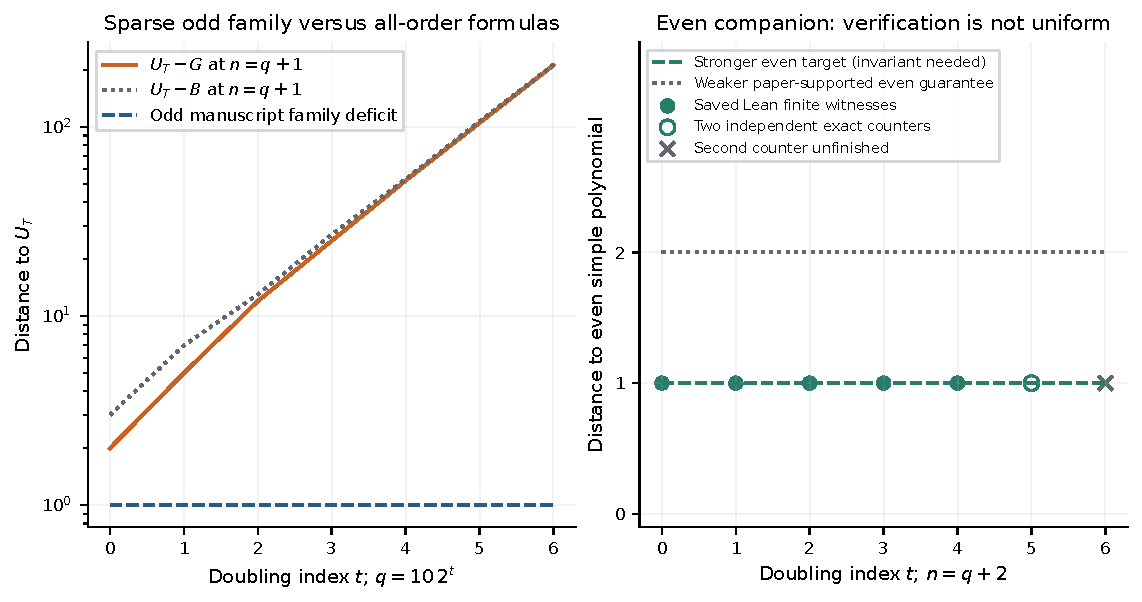
\includegraphics[width=0.88\linewidth]{figures/family-deficits.pdf}
\caption{The sparse hybrid family compared with the all-order baselines.
Odd counts are one below the classical segment bound; the stronger
even checkpoints are one below the displayed simple polynomial bound.
Finite Lean certificates, larger exact coordinate checks, and
family formulas have different verification scopes; the plot does not
turn an incomplete recursive formalization into a proved Lean theorem.}
\label{fig:family-deficits}
\end{figure}

For 321, 322, and 641 lines the adjacency counter and an independently
implemented direct half-plane-sign counter agree on $34132$, $34292$,
and $136532$ triangles, respectively, and simplicity is checked exactly.
The largest rational components have 916, 985, and 1103 decimal digits.
These are archived exact coordinate witnesses, outside the routine
finite Lean catalogue.  The 642-line coordinate file passed the adjacency
and simplicity checks, but its independent direct count was interrupted.
Its displayed value $136852$ is therefore partial computational evidence,
not a completed two-counter or Lean certificate.  No numerical-priority
claim is inferred from these larger files.

\subsection{Known optimal families and independent reproduction}

The classical dyadic five-line family must be kept separate from the
new compatible eleven-line realization.  A convenient normalized seed
uses intercepts $(-1,-\varepsilon,\varepsilon,1)$ and
\[
 x-v_jy=a_j,\qquad (v_0,v_1,v_2,v_3)=(-15,10,-10,30),
\]
together with $Y_0$.  The complete interval
$0<\varepsilon\leq10^{-5}$ has five certified triangles, all three
distinguished triangles, and two visible pairs.  Its central slopes
are $1/10$ and $-1/10$; the rightmost slope is $1/30$.
The normalization is deliberate: an earlier affine-equivalent numerical
realization had both central slopes negative, which was inadequate as
an unchecked premise for the sign convention in the published iterative
proof.  The corrected whole-parameter seed is verified in
\texttt{TamuraSeed5}.

The known optimal odd family and its simple even companions have
\begin{equation}
 q=4\cdot2^t,\qquad
 \Ks(q+1)\geq\frac{q^2-1}{3},\qquad
 \Ks(q+2)\geq\frac{q^2-1}{3}+\frac q2.
 \label{fam:tamura}
\end{equation}
The current finite certificates include
$5:5$, $6:7$, $9:21$, $10:25$, $17:85$, $18:93$, $33:341$,
$34:357$, $65:1365$, $66:1397$, $129:5461$, and $130:5525$.
These reproduce known numerical consequences of the affine family of
Forge and Ram\'irez Alfons\'in and BBL's odd-to-even discussion
\cite{forge1998,bbl2008}; they are not claimed as newly discovered
bounds.  Theorem~\ref{fam:doubling} as currently formalized does not
cover the small bases $q=4,8,16$, and the unfinished large parametric
33-line draft is not counted as a completed theorem.

Parpalak and Utkin supply a different straight-line family at
$q=18\cdot2^t$~\cite{parpalakutkin2026}.  Its odd count is
\begin{equation}
 \Ks(q+1)\geq\frac{q^2}{3}-1,
 \label{fam:pu}
\end{equation}
including $19:107$ and $37:431$.  The present work independently checked
their compatible 19-line seed on $0<\varepsilon\leq10^{-3}$ with 1632
exact endpoint determinant checks, a rational 107-triangle witness,
and all 17 distinguished triangles.  The interval reproduction is
separate from an end-to-end Lean proof of their infinite construction.
Both the seed and the family retain Parpalak--Utkin attribution.
The earlier BBL statement at $18\cdot2^t+1$ concerned pseudolines;
it cannot be used as a straight-line result without a realization
argument.  Applying Corollary~\ref{ext:odd-full} to the published
straight-line family gives the attributed simple even corollary
\[
 \Ks(q+2)\geq\frac{q^2}{3}+\frac q2-1,
\]
with $20:116$, $38:449$, $74:1763$, and $146:6983$.  Stronger nonsimple
published values at some of these orders concern $\K$, and do not
invalidate this simple-arrangement distinction.

\subsection{The exact remaining recursive formalization}

The verified 21-line base has the true tangent intercepts
\eqref{fam:old-grid} with $q=20$, fixed rational slopes, 132 triangles,
19 distinguished triangles, ten visible pairs, and the required
rightmost-line property for every $0<\varepsilon\leq10^{-5}$.
Its finite interval checks use native evaluation; their analytic and
geometric soundness proofs are separately proved.  This is stronger
than a single rational 21-line example.

\begin{figure}[tb]
\centering
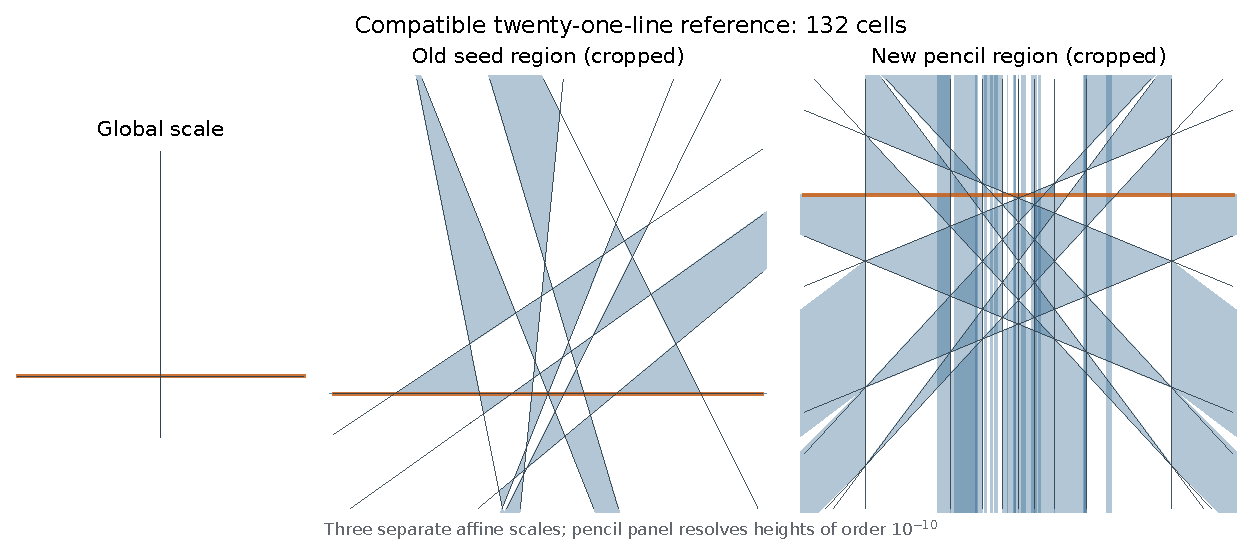
\includegraphics[width=0.88\linewidth]{figures/seed-21.pdf}
\caption{A 21-line hybrid checkpoint with 132 triangles.  The finite
global, core, and thin-pencil views illustrate the scale separation.
The finite rendering is distinct from the true-tangent-grid parametric theorem in
\texttt{BBLSeed21}, which establishes 132 triangles and all 19
distinguished triangles throughout its positive parameter interval.}
\label{fig:seed21}
\end{figure}

Nevertheless, a lower-bound existential statement forgets data needed
by the next step.  The theorem in the library cannot be iterated merely
by substituting its numerical conclusion back into its hypotheses.
The remaining integration has a precise, limited form:
\begin{enumerate}
\item Retain the constructed slopes, the duplicate-free triangle list,
simplicity, distinguished-line saturation, and positive central height
in a recursive seed object.  Select $\kappa$ to preserve the central
triangle independently of the counted list, since that list may omit it.
\item Sort the old and new intercepts into the next grid.  The explicit
permutation and tangent-cut identity are proved in
\texttt{BBLGridReindex}.  The next distinguished triangles are proved
in \texttt{BBLNextSaturation}: each noncentral interval is one of the
mixed triangles, and the central interval uses the retained central
triangle.  Whole-list transport must still supply all support
permutations, preserve distinctness and length, and identify the
reindexed graph equations.
\item Normalize the grouped labels of \texttt{BBLSeed21} into increasing
intercept order.  Its central source labels are 5 and 6, whose apex has
height $5\varepsilon/2$, so positivity follows without another interval
search.  The sorting permutation leaves the central old supports in
place geometrically; hence the next central apex is exactly the old
one, not merely close to it.
\item Induct on a uniform small-parameter existence statement
\begin{equation}
 \exists\eta>0\quad\forall\varepsilon\in(0,\eta)\quad
 \exists\text{ a compatible counted seed at }(q,\varepsilon).
 \label{fam:recursive-quantifier}
\end{equation}
At the next stage shrink $\eta$ below the needed half-grid gap.  The
slopes, $\delta$, and $\kappa$ may depend on $\varepsilon$.
\end{enumerate}
The sought closure is, schematically,
\[
 \operatorname{Compatible}(r,\varepsilon,T)
 \Longrightarrow
 \operatorname{Compatible}(2r,\varepsilon,T+(4r)^2)
\]
under $r\geq5$ and \eqref{fam:epsilon}.  This is a proposed theorem
interface, not a declaration already present in the checked library.
Starting from 21 lines would give the formal target
\begin{equation}
 q_t=20\cdot2^t,\qquad
 \Ks(q_t+1)\geq\frac{q_t^2-4}{3}.
 \label{fam:21-target}
\end{equation}
Numerically this is the tail of \eqref{fam:eleven-family}.  Its purpose
is to close the formal geometric dependency, not to establish another
numerical priority claim.  The stronger even family further requires
the separate visibility invariant of
Proposition~\ref{fam:even-conditional}.

A bounded search for a compatible perfect 21-line seed did not improve
132: it tested 11547910 floating proposals, with exact checking reserved
for any prospective 133-triangle result, and found none.  A separate
3234-program linear-feasibility transfer search likewise found no strict
feasible margin.  These are reproducible negative search results,
consistent with the compatibility difficulties discussed in
\cite{parpalakutkin2026}; neither proves nonexistence.  Improving a
compatible seed, finding a useful partial-doubling interpolation, and
closing the recursive invariant remain different research problems.

\section{Multiplicity-sensitive upper-bound arguments}
\label{upper:scope}

This section develops restricted upper estimates by separating the ordinary part of an arrangement from its finite multiple points. The geometric derivations below are ordinary mathematical proofs. The local fan geometry and cyclic counting are formalized in Lean, while the extraction of elementary segments from an arbitrary arrangement and the global clean-line charging argument are not. Accordingly, this section does not assert a completed Lean upper theorem for all arrangements, and none of its restricted conclusions is an improved upper bound for the full function $\K$.

The distinction is necessary because the even-order estimates of Bartholdi--Blanc--Loisel and Blanc require simplicity~\citep{bbl2008,blanc2011}. The classical Cl\'ement--Bader envelope is treated as a reported external theorem~\citep{clementbader2007}; the local example in Section~\ref{upper:shared-fan} explains why we do not silently replace its proof by a bound on all shared edges incident to a multiple point.

\subsection{An exact elementary-segment identity}

\begin{definition}
For an arrangement of $n$ distinct affine lines, let $t_r$ be the number of finite intersection points incident to exactly $r$ lines, and let $P$ be the number of unordered parallel pairs. A bounded \emph{elementary segment} is the portion of an arrangement line between two consecutive finite intersection points. Let $E$ count these segments, $U$ count those incident to no triangular cell, and $D$ count those incident to two triangular cells. Let $a$ be the number of lines containing at least one finite intersection point, and put
\[
 S=\sum_{r\ge3}r(r-2)t_r,\qquad
 \delta=n(n-2)-3T,
\]
where $T$ is the number of bounded triangular cells.
\end{definition}

\begin{proposition}[Segment and defect identities]
\label{upper:identity}
For every such arrangement,
\begin{align}
 E&=n(n-1)-2P-S-a,\\
 3T&=E-U+D,\\
 \delta&=2P+S+a-n+U-D.
 \label{upper:defect-general}
\end{align}
If every line meets another line, then $a=n$ and $\delta=2P+S+U-D$.
\end{proposition}

\begin{proof}
Each nonparallel unordered pair contributes to exactly one finite point, so
\[
 n(n-1)-2P=\sum_{r\ge2}r(r-1)t_r.
\]
If a line has $s>0$ distinct finite intersection points, it contributes $s-1$ bounded elementary segments; an isolated line contributes none. Summing point-line incidences gives
\[
 E=\sum_{r\ge2}r t_r-a.
\]
Subtracting these expressions yields the first identity. Each triangular cell uses three elementary segments. A segment is incident to zero, one, or two such cells, so the total number of triangle-side incidences is $E-U+D$. Substitution into the definition of $\delta$ gives the last identity.
\end{proof}

The term $D$ cannot be dropped in a nonsimple arrangement. Multiple points reduce the available segment count by $S$, but sharing can compensate for some of that loss. This is precisely the interaction that a classical upper proof must control.

\begin{lemma}[A shared side has a multiple endpoint]
\label{upper:shared-endpoint}
An elementary segment incident to two bounded triangular cells cannot have both endpoints ordinary, where an ordinary point is incident to exactly two arrangement lines.
\end{lemma}

\begin{proof}
At each ordinary endpoint there is a unique supporting line other than the line containing the segment. Both adjacent triangles would therefore have the same three supporting lines. Three distinct lines have at most one bounded triangular region, whereas the two incident cells lie on opposite sides of the shared segment. This is impossible.
\end{proof}

For the remainder of the section assume that $n\ge4$ is even and that all pairs of lines are nonparallel. Let the \emph{core} consist of the finite points of multiplicity at least three. Write
\[
 q=\sum_{r\ge3}t_r,\qquad I=\sum_{r\ge3}r t_r,
\]
and let $h$ count the lines meeting the core. Let $D_1$ count shared elementary segments with exactly one core endpoint and $D_2$ those with two core endpoints. By Lemma~\ref{upper:shared-endpoint}, $D=D_1+D_2$, and hence
\begin{equation}
 \delta=S+U-D_1-D_2.
 \label{upper:core-identity}
\end{equation}

\subsection{Parity on a line outside the core}

A line is \emph{clean} if it contains no core point. The following argument adapts the local parity method in Blanc's Section~2~\citep{blanc2011}. Its proof is included because the transverse lines may have multiple intersections away from the clean line.

\begin{lemma}[Clean-line charging]
\label{upper:clean-charge}
For even $n\ge4$ and pairwise nonparallel lines,
\begin{equation}
 n-h\le2U+D_1.
 \label{upper:charging}
\end{equation}
\end{lemma}

\begin{proof}
First fix a clean line $L$, place it horizontally, and number its $n-1$ crossings from left to right. Let $R_i$ be the transverse line at crossing $i$. Denote the bounded segment of $L$ between crossings $i$ and $i+1$ by $\ell_i$, and its two exterior rays by $\ell_0$ and $\ell_{n-1}$. Write $p_i^+$ and $p_i^-$ for the faces above and below $\ell_i$, and $r_i^+,r_i^-$ for the elementary transverse pieces of $R_i$ immediately above and below $L$. A transverse piece may be a bounded segment or an unbounded ray.

We show that some bounded $r_i^{\pm}$ is unused or shared. Suppose otherwise: every bounded transverse piece is incident to exactly one triangle. Each bounded $\ell_i$ is unshared by Lemma~\ref{upper:shared-endpoint}.

If both $p_1^+$ and $p_1^-$ are nontriangular, then $r_1^+$ and $r_1^-$ are unused: their other adjacent faces meet the exterior ray $\ell_0$. At least one of these transverse pieces is bounded, because $R_1$ meets another transverse line. This contradicts the supposition. Reflecting across $L$ if necessary, assume $p_1^+$ is triangular; $p_1^-$ is then not.

For $1\le i\le n-2$, prove the following assertions together:
\begin{enumerate}[label=(\roman*)]
\item if $i$ is even, $p_i^+$ is nontriangular; if $i$ is odd, $p_i^-$ is nontriangular;
\item if both faces at $\ell_{i-1}$ are nontriangular, then $p_i^-$ is triangular for even $i$, and $p_i^+$ is triangular for odd $i$.
\end{enumerate}
The base case follows from the choice of $p_1^+$ and the unbounded faces at $\ell_0$. Consider an even step; the odd step exchanges signs. If $p_{i-1}^+$ is triangular, then $p_i^+$ cannot be triangular, since otherwise the two triangles share the bounded piece $r_i^+$, contrary to the supposition. Assertion (ii) has a false antecedent in this case.

Otherwise both $p_{i-1}^+$ and $p_{i-1}^-$ are nontriangular by the preceding odd step. This cannot happen for $i=2$, so $i\ge4$. The earlier even step makes $p_{i-2}^+$ nontriangular. Hence $r_{i-1}^+$ is unused, and must be unbounded. The intersection of $R_{i-1}$ and $R_i$ must consequently lie below $L$. It follows that $r_i^-$ is bounded. Its left adjacent face is nontriangular, so its right adjacent face $p_i^-$ must be triangular. Since $\ell_i$ is unshared, $p_i^+$ is nontriangular. This proves both assertions.

Now $n-2$ is even, so $p_{n-2}^+$ is nontriangular. If $p_{n-2}^-$ is also nontriangular, both pieces at the last crossing are unused and at least one is bounded, again a contradiction. Otherwise $p_1^+$ and $p_{n-2}^-$ are triangular, while $r_1^-$ and $r_{n-1}^+$ are unused. The lines $R_1$ and $R_{n-1}$ intersect. If their intersection is below $L$, then $r_1^-$ is bounded; if above, then $r_{n-1}^+$ is bounded. This is the final contradiction.

Charge each clean line to one bounded unused or shared transverse segment supplied by this argument. An unused segment can receive at most two charges, one at each ordinary endpoint. A shared segment must have a multiple endpoint, so it can receive at most one charge if counted by $D_1$, and none if counted by $D_2$. There are $n-h$ clean lines, giving~\eqref{upper:charging}.
\end{proof}

\begin{remark}[Why parallel pairs have been excluded]
Three parallel vertical lines and one horizontal line give a clean horizontal line whose transverse pieces are all unbounded. Thus simply removing parallel-participating lines from the set to be charged does not prove the lemma. The identities of Proposition~\ref{upper:identity} allow parallels, but the charging argument above does not. Every subsequent upper estimate in this section retains the pairwise nonparallel hypothesis.
\end{remark}

Combining~\eqref{upper:core-identity} and~\eqref{upper:charging} gives the basic budget
\begin{equation}
 2\delta\ge n+2S-h-3D_1-2D_2.
 \label{upper:basic-budget}
\end{equation}
The remaining problem is to bound the shared-side contribution at the core.

\subsection{The geometric obstruction in a cyclic fan}

At an $r$-fold point $v$, the incident lines determine $2r$ rays in cyclic order, with opposite rays separated by $r$ positions. Let $d_1(v)$ count shared elementary segments starting at $v$ and ending at an ordinary point, and let $d_2(v)$ count those ending at another core point. A ray supports at most one such incident elementary segment.

\begin{lemma}[No long run of ordinary-ended shared rays]
\label{upper:no-long-run}
For $r\ge3$, no $r-1$ consecutive rays at an $r$-fold point can all support segments counted by $d_1(v)$.
\end{lemma}

\begin{proof}
Such a run would border $r$ consecutive triangular sectors. At the ordinary endpoint of each selected shared segment, the opposite supporting lines of the two neighboring triangles must coincide: besides the radial line through $v$, only one arrangement line passes through that endpoint. Propagating this equality makes the opposite sides of all $r$ triangles lie on one line $M$.

The line $M$ would meet $r+1$ consecutive rays from $v$, which include an opposite pair. A line meeting both open opposite rays must contain their connecting segment and hence $v$. But the opposite side of a nondegenerate triangle with vertex $v$ cannot lie on a line through $v$. This contradiction proves the lemma.
\end{proof}

This is an actual geometric statement, not an assumed combinatorial prohibition. The Lean module \texttt{FanGeometry} proves uniqueness and propagation of opposite supports for real lines and points. The module \texttt{CyclicFan} supplies the cyclic-to-geometric bridge from triangular sectors, antipodal rays and ordinary selected endpoints.

\begin{proposition}[Local fan budget]
\label{upper:fan-budget}
At every finite point of multiplicity $r\ge3$,
\begin{equation}
 d_1(v)\le2r-3,\qquad 3d_1(v)+d_2(v)\le6r-6.
 \label{upper:local-fan-budget}
\end{equation}
\end{proposition}

\begin{proof}
Count selected rays in all $2r$ cyclic windows of length $r-1$. Each window contains at most $r-2$ selected rays by Lemma~\ref{upper:no-long-run}, and each selected ray belongs to exactly $r-1$ windows. Therefore
\[
 (r-1)d_1(v)\le2r(r-2).
\]
If $d_1(v)\ge2r-2$, the left side is at least $2(r-1)^2=2r(r-2)+2$, a contradiction. Finally $d_1(v)+d_2(v)\le2r$, so
\[
 3d_1(v)+d_2(v)=2d_1(v)+(d_1(v)+d_2(v))\le6r-6.
\]
\end{proof}

The cyclic double count is proved in \texttt{FanCount}. The theorem \lean{CyclicFan.selected_card_le} combines it with the real geometric obstruction, without assuming the no-long-run conclusion as an unexplained premise.

\subsection{A weighted bound for an arbitrary finite core}

\begin{proposition}[Multiplicity-weighted defect estimate; manuscript geometry]
\label{upper:weighted}
Let $n\ge4$ be even and let the arrangement be pairwise nonparallel. Then
\begin{equation}
 2\delta\ge n+\sum_{r\ge3}(2r^2-11r+6)t_r.
 \label{upper:weighted-defect}
\end{equation}
\end{proposition}

\begin{proof}
Each $D_1$ segment has exactly one core endpoint and each $D_2$ segment has two. Summing~\eqref{upper:local-fan-budget} gives
\[
 3D_1+2D_2\le6I-6q.
\]
Also $h\le I$, since every core line contributes at least one point-line incidence. Inserting both inequalities into~\eqref{upper:basic-budget} yields
\[
 2\delta\ge n+2S-7I+6q,
\]
which is~\eqref{upper:weighted-defect} after expanding $S,I,q$.
\end{proof}

The local weights are $-9,-6,1,12,27$ at multiplicities $3,4,5,6,7$, respectively. Consequently the obstruction to recovering a simple-style parity defect is concentrated at triple and quadruple points; higher multiplicity has a positive weight in this accounting.

\begin{corollary}[Nonnegative core weight; manuscript geometry]
\label{upper:high-multiplicity}
Under the hypotheses of Proposition~\ref{upper:weighted}, if
\[
 \sum_{r\ge3}(2r^2-11r+6)t_r\ge0,
\]
then
\[
 T\le\left\lfloor\frac{n(n-5/2)}3\right\rfloor.
\]
In particular, this holds if every finite multiple point has multiplicity at least five.
\end{corollary}

\begin{proof}
The weighted estimate implies $\delta\ge n/2$, giving the displayed upper bound by the definition of $\delta$. For $r\ge5$, the exact factorization
\[
 2r^2-11r+6=1+(r-5)(2r-1)\ge1
\]
proves the stated sufficient condition.
\end{proof}

This extends the same polynomial to a restricted nonsimple class. It says nothing comparable for a general core consisting of many triple points. Numerical first priority for this restricted consequence has not been established.

\subsection{A sharper estimate with at most two core points}

\begin{lemma}[A fan with at most one core-to-core ray]
\label{upper:one-core-ray}
If $d_2(v)\le1$ at a point of multiplicity $r\ge3$, then $d_1(v)\le2r-4$.
\end{lemma}

\begin{proof}
Mark which of the $2r$ sectors at $v$ are triangular. A ray supports a shared elementary segment exactly when both neighboring sectors are triangular. If every sector is triangular, every ray is shared; deleting at most one $d_2$ ray leaves a run of at least $2r-1$ selected rays, contradicting Lemma~\ref{upper:no-long-run}. Hence a nontriangular sector exists.

Suppose $d_1(v)\ge2r-3$. Two separated nontriangular sectors exclude at least four shared rays, as do three consecutive nontriangular sectors. Both situations are impossible. If exactly one sector is nontriangular, the shared rays form a path of length $2r-2$. Deleting at most one $d_2$ ray leaves at most two selected runs. Their total capacity is $2(r-2)$, less than the required $2r-3$. If exactly two adjacent sectors are nontriangular, at most $2r-3$ shared rays remain. All would have to be selected, forming a run of length $2r-3>r-2$. These cases exhaust the possibilities and prove the lemma.
\end{proof}

\begin{theorem}[At most two finite multiple points; manuscript geometry]
\label{upper:two-core}
An arrangement of an even number $n\ge4$ of pairwise nonparallel affine lines with at most two finite multiple points satisfies
\begin{equation}
 T\le\left\lfloor\frac{n(n-5/2)}3\right\rfloor+1.
 \label{upper:two-core-upper}
\end{equation}
More precisely, the defect bounds are $\delta\ge n/2$ if $q=0$, $\delta\ge n/2-1$ if $q=1$, and $\delta\ge n/2-3$ if $q\le2$.
\end{theorem}

\begin{proof}
With at most two core points, at most one ray at a core point can terminate at another core point. Lemma~\ref{upper:one-core-ray} gives $D_1\le2I-4q$. There is at most one core-to-core shared segment, so $D_2\le q(q-1)/2\le1$. Moreover,
\[
 h\le I-D_2,
\]
because any such segment lies on a line counted twice in the core-incidence total and once among the core lines. Substitution in~\eqref{upper:basic-budget} yields
\[
 2\delta\ge n+\sum_{r\ge3}(2r^2-11r+12)t_r-D_2.
\]
For $r\ge3$,
\[
 2r^2-11r+12=-3+(r-3)(2r-5)\ge-3.
\]
Thus $2\delta\ge n-3q-D_2\ge n-7$. Since $n$ and $2\delta$ are even, $2\delta\ge n-6$. Rearranging gives~\eqref{upper:two-core-upper}. If $q=1$, then $D_2=0$ and the inequality $2\delta\ge n-3$ rounds to $2\delta\ge n-2$; if $q=0$, it gives $2\delta\ge n$ directly.
\end{proof}

The hypotheses are attained by externally attributed exact constructions. Table~\ref{upper:restricted-attainment} records examples whose pairwise nonparallel status, triangle count, and two triple points were checked exactly. Their equality with~\eqref{upper:two-core-upper} proves sharpness within this restricted class, not optimality over all classical arrangements.

\begin{table}[htbp]
\centering\small
\begin{tabular}{@{}rrrl@{}}
\toprule
$n$ & $T$ & Restricted upper & Coordinate provenance\\
\midrule
8 & 15 & 15 & Earlier construction, retained in the current gallery\\
14 & 54 & 54 & Maiorana, two-triple-point witnesses\\
26 & 204 & 204 & Parpalak--Utkin gallery\\
50 & 792 & 792 & Parpalak--Utkin gallery\\
\bottomrule
\end{tabular}
\caption{Attainment in the class covered by Theorem~\ref{upper:two-core}. Sources: \citet{maiorana2026,parpalakutkinGallery2026}. These are not new numerical records claimed by this paper.}
\label{upper:restricted-attainment}
\end{table}

ProofAtlas reports a stronger restriction-specific result at $n=14$, covering up to four finite multiple points~\citep{proofatlas2026}. Its proof was not independently reproduced here. Our two-point estimate covers all even orders and arbitrary core multiplicities, but neither that fact nor the table establishes priority for the restricted theorem.

\subsection{A checked shared-fan example and the limits of smoothing}
\label{upper:shared-fan}

Consider the six lines
\begin{equation}
 x=0,\quad y=0,\quad x+y=3,\quad x-y=0,\quad
 2x+y=3,\quad x+2y=3.
 \label{upper:median-lines}
\end{equation}
They are the three sides of a triangle and its three medians. There are six bounded triangular cells and four triple points. At $v=(1,1)$, six distinct nonzero elementary radial segments are shared sides, each belonging to two of those cells. Three have ordinary other endpoints and three have multiple other endpoints, giving $d_1(v)=d_2(v)=3$; globally $D_1=D_2=3$.

\begin{figure}[htbp]
\centering
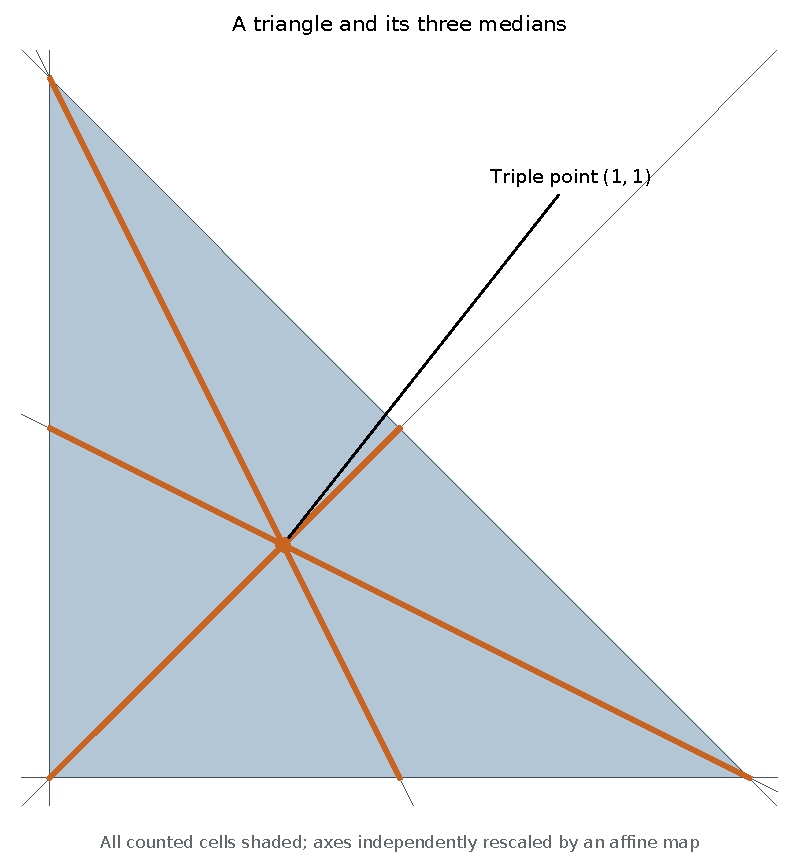
\includegraphics[width=0.75\textwidth]{figures/shared-fan.pdf}
\caption{The exact arrangement~\eqref{upper:median-lines}. Six triangular cells meet around the central triple point, and all six radial sides are shared. This refutes only a literal local incidence reading of the shared-pair statement in Cl\'ement--Bader's Lemma~1; it does not refute their final upper theorem. The figure is newly generated from the integer equations.}
\label{fig:shared-fan}
\end{figure}

The \texttt{SharedFan} module proves the real geometric facts: each designated triangle has nonempty uncut interior, the six interiors are pairwise disjoint, the radial segments are distinct and elementary, and each is a side of two distinct triangles. The proof uses ordinary kernel checking.

This matters when interpreting the Cl\'ement--Bader proof. Its local shared-pair sentence cannot literally bound all shared segments incident to a multiple point by two. An intended assignment of each shared side to one endpoint would be a different assertion requiring global justification. The example has only six triangles, below the reported seven-triangle upper bound at order six; it is therefore not a counterexample to that upper theorem. The present paper leaves that distinction explicit and uses the separate $D_1,D_2$ accounting instead.

Nor can one justify a simple upper bound merely by perturbing every multiple point. For a retained two-triple-point Maiorana $14{:}54$ witness, the four local generic resolution types have triangle counts $52,52,53,52$. These counts were checked with exact arithmetic; they are finite experimental evidence, not a new Lean theorem classifying all perturbations. They demonstrate why a universally nondecreasing smoothing argument needs more than the existence of a small generic perturbation. Our global upper argument never assumes such monotonicity.

\subsection{Formal status and the remaining bridge}

The following division is part of the mathematical claim, not an implementation footnote.
\begin{table}[htbp]
\centering\small
\begin{tabularx}{\textwidth}{@{}lXX@{}}
\toprule
Module or argument & Completed & Still required for a global Lean upper theorem\\
\midrule
\texttt{SharedFan} & Exact real six-line counterexample to the literal local reading. & No general conclusion is inferred from this example.\\
\texttt{FanGeometry} & Uniqueness and propagation of opposite supports; obstruction at opposite rays. & Extract fan strips from arbitrary arrangement cells.\\
\texttt{FanCount} & Cyclic-window double count and $2r-3$ bound. & Supply its geometric selected set.\\
\texttt{CyclicFan} & Actual sector geometry implies the no-long-run property and selected-cardinality bound. & Construct the cyclic sector data globally.\\
\texttt{CleanLineBudget} & Integer consequences of explicitly supplied incidence, charging, and fan inequalities. & Prove those hypotheses for all arrangements in the intended class.\\
Paper-level geometry & Segment identity, clean-line parity charging, and restricted consequences above. & Formal elementary edges, their cell incidences, global summation, and the sharper $d_2\le1$ fan refinement.\\
\bottomrule
\end{tabularx}
\caption{The upper-bound formalization boundary. Every completed module in this table was checked without placeholders; the table does not identify the conditional arithmetic module with a completed geometric upper theorem.}
\label{upper:formal-status}
\end{table}

In particular, \texttt{CleanLineBudget} also contains arithmetic implications with a symbolic parallel-pair term. Those implications do not prove the missing charging lemma with parallels. The nine conditional arithmetic theorems and the geometric fan modules use only the standard axiom set recorded for this development. Exact finite checks on $597$ test arrangements, followed by the imported Maiorana and gallery witnesses, support the accounting and expose implementation mistakes; they do not replace its general proof.

The main unresolved direction is therefore precise. One must control the negatively weighted triple and quadruple points, account for the entire core rather than a chosen subgraph, and separately handle parallel classes. Completing the global Lean extraction would certify the restricted results above. Improving the unrestricted numerical upper envelope requires an additional mathematical idea beyond those formalization tasks.

\section{Exact certificates, external reproduction, and unsuccessful searches}
\label{exp:section}

The experimental program serves two purposes: producing concrete coordinate
witnesses for lower bounds, and identifying which proposed general arguments
survive exact checks. These purposes require different standards of evidence.
A successful coordinate witness proves an existential lower bound at its
specified order. A failed search ordinarily proves neither an upper bound nor
the nonexistence of a better construction. This section records both positive
and negative outcomes without merging their logical scopes.

\subsection{From a numerical proposal to an exact geometric witness}

The stored coordinates use the convention $a_ix+b_iy=c_i$, with rational or
integer coefficients. Each line is normalized to a primitive integer triple.
Pair intersections are computed as homogeneous integer triples, normalized
with a positive final coordinate. Consequently, collinearity, concurrence,
parallelism, and comparisons along a supporting line can all be tested without
floating-point tolerances.

Two independently implemented counters are used. The first sorts the distinct
intersection vertices on each line and constructs the graph of elementary
bounded segments; a three-cycle supported by three different lines is a
triangular cell. The second enumerates support triples and tests whether every
other line has a common weak sign at their three vertices. Nonzero area and
the distinction between open interiors and boundaries are checked explicitly.
Where a complete independent verification is reported, both counters agree on
the triangle set, not merely on a rounded area or a visual estimate. The Lean
geometric soundness theorem provides a third, logically separate link from
accepted coordinate predicates to real affine triangles.

Numerical optimization is used only to propose coordinates or rank candidate
chambers. A proposal is rationalized and recounted before promotion. In the
phase/chart experiments, progressively finer integer scales were accepted only
when the entire exact triangle set and simplicity were retained. Such a finite
acceptance does not prove that an arbitrary rounding of an irrational
construction is valid. The real all-order theorem for $\G$ has its own
determinant, trigonometric, and counting proof.

The released catalog contains 138 distinct promoted coordinate identities.
Several identities can occur at the same order and triangle count, and an
identity may have several repository source paths. Thus 138 is a catalog size,
not a count of new records or independent discoveries. The complete catalog
in Table~\ref{exp:catalog} includes simple versus nonsimple status, provenance
collections, and coordinate-hash prefixes; its machine-readable companion
records full hashes, source paths, and theorem modules. The finite Lean
certificates use native evaluation where indicated. This trust boundary is
broader than that of the universal construction, whose proof uses only Lean's
standard logical axioms.

\subsection{Finite improvements relative to the retained collection}

The phase and affine-chart work raised the preceding saved values at eleven
orders:
\[
\begin{array}{c|rrrrrrrrrrr}
n&39&47&48&51&53&54&55&59&60&99&195\\\hline
\text{previous}&469&690&720&817&884&918&954&1102&1140&3169&12481\\
\text{current}&470&691&721&818&885&919&955&1103&1141&3170&12482
\end{array}
\]
Each row is an improvement over the project's preceding retained coordinate
catalog. The underlying trigonometric family is due to
F\"uredi--Pal\'asti~\cite{furedipalasti1984}; these comparisons do not establish
numerical first priority. The general formula $\G$ now explains all eleven
displayed counts. The first projective search reached $47:691$ after 11,264
proposals; the subsequent exposed-cap description replaced that search by a
direct construction and an all-order proof.

The earlier OEIS-attributed values $28:238$, $30:275$, and $34:357$ remain
independently certified~\cite{oeisA006066,zarzuelo2026}. The drawings in this
paper render the currently retained exact witnesses, obtained by exterior
extension of retained odd-order inputs. They are not asserted to be literal
reproductions of the March diagrams. Likewise, the historical inventory in
Table~\ref{exp:historical} preserves earlier outputs without upgrading every
original derivation to a completed general theorem.

The current strongest saved simple and classical coordinate counts for every
$3\leq n\leq60$ appear in Table~\ref{exp:finite-table}. An absent entry in the
explicit OEIS table is recorded as a dash. Absence from that table is not
evidence that a value is absent from the literature; conversely, a coordinate
certificate does not establish optimality without an upper theorem covering
the same arrangement class.

\subsection{Independent reproduction of external constructions}

The current Parpalak--Utkin coordinate gallery~\cite{parpalakutkin2026} supplied
exact witnesses at
\[
\begin{gathered}
8:15,\quad14:54,\quad20:117,\quad26:204,\quad32:315,\\
36:402,\quad38:450,\quad42:553,\quad46:667,\quad50:792.
\end{gathered}
\]
Both independent counters reproduced their triangle sets. These witnesses
retain their source attribution; in particular, the eight-line numerical
value has older discovery priority than the coordinate gallery. Their addition
to this repository improves its verified coverage, not the discoverer's
claim to the numbers. The inspected gallery snapshot is commit
\texttt{feae4f5571a988a3ed45bd26a36259ebb7d7d3d2}.

All fifteen of Andrea Maiorana's published $14:54$ coordinate
configurations~\cite{maiorana2026} were also independently checked. Fourteen
have exactly two triple points, and one has four; none has a parallel pair.
The source snapshot is commit
\texttt{e47c7cfd9661e54d29befb83118bf83d5f804028}. Its CC BY 4.0 licence,
original coordinate files, and source attribution are retained. Added wrappers
record counts and verification metadata. This reproduction imports no claim
that a simple-arrangement upper theorem applies to these nonsimple witnesses.

These examples also expose a concrete limitation of smoothing. In Maiorana's
first example, the triple supports are $\{0,4,10\}$ and $\{0,11,12\}$.
Independently shifting the offsets of lines 4 and 11 by $\pm1/1000$ realizes all
four local resolution choices while preserving every originally nonzero
determinant sign. The resulting triangle counts are $52,52,53,52$, all below
54. Thus the proposed nondecreasing local smoothing strategy fails even when
the local sign choices are independently realizable by straight lines. The
argument identifying these sign choices with all sufficiently small local
resolutions is an ordinary finite sign-stability argument, not a completed
Lean theorem.

For the gallery's collinear-core examples at orders
$8,14,20,26,32,38,50$, all 132 recorded local resolutions were realized by
exact private-line offsets. Their respective best simple counts were
$14,51,114,203,313,448,791$. In particular, a universal claim that resolving
such a core loses at most one triangle is also false. Figure~\ref{fig:external-comparison}
separates these finite obstructions from any general upper-bound assertion.

\begin{figure}[tbp]
  \centering
  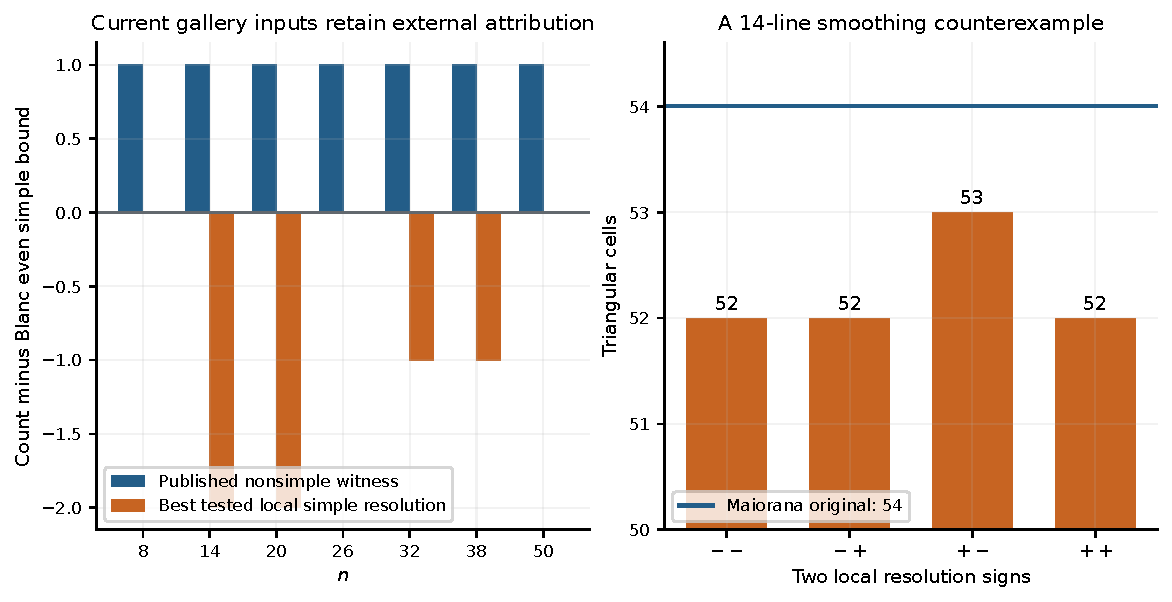
\includegraphics[width=\textwidth]{figures/external-comparison.pdf}
  \caption{Exact local-resolution tests on attributed external constructions.
  Left: Parpalak--Utkin gallery witnesses and their best tested simple local
  resolutions, measured relative to Blanc's even simple-arrangement polynomial;
  the eight-line value has older priority. Right: all four local resolutions of
  Maiorana's two-triple-point $14:54$ example. The original arrangements are
  nonsimple, so exceeding the simple polynomial is consistent. These are
  smoothing obstructions, not upper bounds for the classical problem.}
  \label{fig:external-comparison}
\end{figure}

\subsection{Projective charts, algebraic curves, and chamber searches}

Projective geometry provides a useful global neighborhood: changing the line
at infinity moves all lines together and may bound formerly unbounded
triangular faces. It can also lose bounded cells. For the exact saved
$81:2132$ and $161:8532$ hybrid arrangements, the projective triangular-face
census already equals their bounded-cell count; a chart change alone cannot
increase those particular counts.

Exact rational linear-arithmetic searches give sharper restrictions for some
fixed configurations. The nine-line half-phase rational arrangement has 21
projective triangular faces, but the recorded QF\_LRA solver result rules out a
chart retaining all 21. Similar fixed-seed tests find no gain for the tested
half-phase arrangements at $14,20,26,44$, and no chart retaining all 471
projective triangles of the saved $39:470$ witness. For a nonuniform cubic
48-line seed with 724 projective triangles, 2,903 exact linear-arithmetic checks
rule out 722 bounded triangles within the tested chart-retention formulation.
These are exact-solver results about specified rational seeds. Their UNSAT
certificates have not been independently checked in Lean, and they are not
global upper bounds at those orders.

The algebraic-curve direction tested both nodal-cubic angle perturbations and
torsion cosets on real elliptic curves. A larger projective face count did not
automatically produce a better affine construction. For the better two-real-
component elliptic examples, the projective, original affine, and best found
affine counts were respectively
\[
\begin{array}{c|rrrr}
n&42&48&54&60\\\hline
\text{projective}&550&724&922&1144\\
\text{original affine}&538&710&907&1127\\
\text{best found affine}&539&712&908&1129
\end{array}
\]
All fall below the corresponding retained affine bounds. The chart scans at
54 and 60 had 90-second limits. Numerical ranking and bounded running time
preclude a global nonexistence inference.

Oriented-matroid mutations and kinetic chamber sweeps addressed a different
limitation: moving inside a fixed projective type cannot create new
projective triangular faces. The mutation searches changed determinant signs,
using linear-programming realization where appropriate. Kinetic sweeps varied
many offsets, or both slopes and offsets, and visited concurrency events along
selected rays. Their event counts are not counts of all realizable order
types, and unsuccessful floating rays were discarded. Figure~\ref{fig:negative-searches}
records effort without treating heterogeneous search units as comparable
coverage measures.

\begin{figure}[tbp]
  \centering
  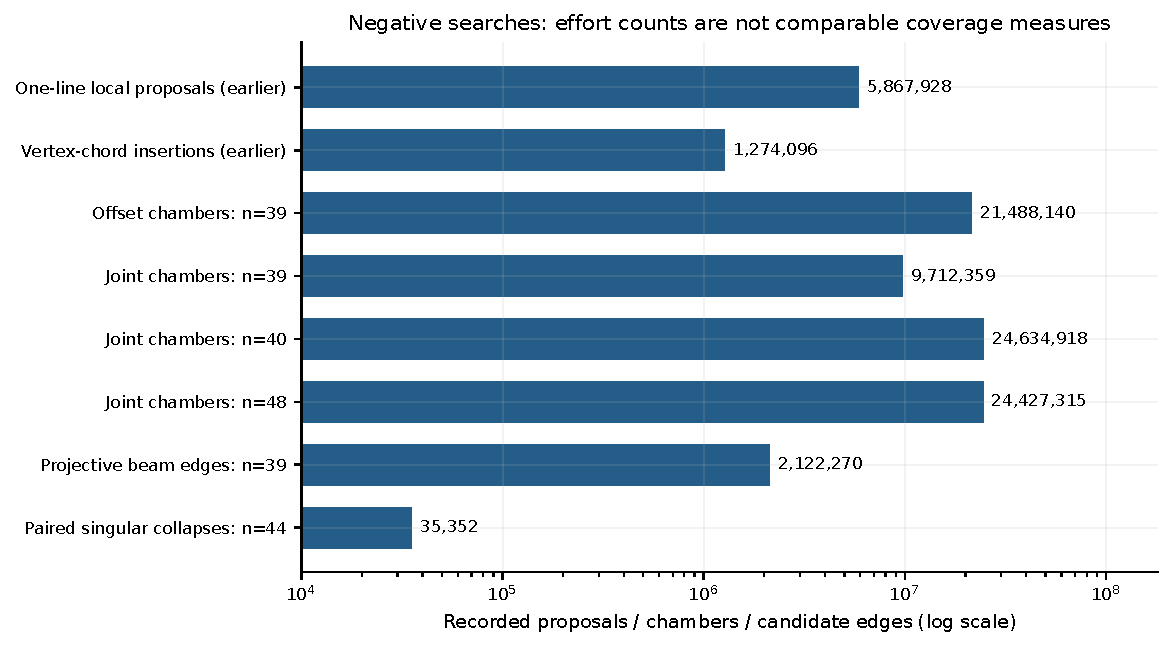
\includegraphics[width=\textwidth]{figures/negative-searches.pdf}
  \caption{Selected unsuccessful searches, with their recorded units.
  Proposal, chamber, and candidate-edge totals describe different search
  neighborhoods. They do not measure exhaustive coverage, justify an upper
  bound, or rank the mathematical promise of the methods. All proposed
  improvements would require subsequent exact geometric verification.}
  \label{fig:negative-searches}
\end{figure}

The final 39-line projective beam examined 2,122,270 candidate edges through
4,559 states without exceeding 470 affine or 471 projective triangles, even
at its combinatorial scoring stage. The 48-line LP walk accepted 471 mutations
out of 511 attempts and retained 721 affine and 724 projective triangles.
At 44 lines, singular-boundary searches included 35,352 paired collapses;
the retained beam checkpoint had 771 states and 446,422 candidate edges,
without exceeding 608. An unfinished round was discarded. These results
motivate a change of neighborhood or a structural argument rather than
repeating the same local searches.

Other bounded approaches included Fourier deformations (2,687,600 proposals
in one 39-line run), partial deletions from BBL constructions, and constrained
tangent-grid transfer by LP/MILP. The tested optimal 23-line chart transfers
did not admit a positive-margin realization on the desired grid; a constrained
near-optimal search gave 144 triangles, below a separately known compatible
145. None of these observations proves nonexistence of another compatible
seed or a different successful deletion pattern.

\subsection{Reproduction and presentation audit}

The research registers preserve source snapshots, experiment scripts, seeds,
parameters, checkpoints, and exactness limits~\cite{zarzueloRepository}. The
paper's figures are original vector renderings, not copied source figures.
The generator \texttt{paper/scripts/generate\_figures.py} reads the research
data without modifying it and exports PDF figures, PNG previews, LaTeX tables,
and machine-readable rendering data. The figure manifest records input-file
hashes and the mathematical status of each caption. Geometric views recompute
their exact triangle lists before converting coordinates to floating point
for display. Cropped detail panels and independent affine axis rescaling are
explicitly labeled; lengths and angles are not inferred from those views.

The appropriate experimental conclusion is therefore selective. Exact
coordinates have strengthened the retained lower-bound envelope and revealed
specific failed construction rules. The successful universal advance comes
from replacing a numerical chart search by a geometric exposure proof and an
all-order count. The remaining negative searches narrow useful next steps,
but they do not solve the general optimization problem.

\section{Formal verification and reproducibility}\label{sec:formalization}

\subsection{The verified snapshot}

The mathematical snapshot used by this paper is repository commit
\nolinkurl{99fdc8ec1ef8b1fb22c3da32b011b7361762e958}. It pins Lean 4.31.0 and Mathlib commit
\nolinkurl{fabf563a7c95a166b8d7b6efca11c8b4dc9d911f}. The local release audit completed on 22 September 2026, and the independent GitHub Actions run 35699093671 subsequently passed. These are reproducibility statements about a particular collection of declarations and coordinates, not an assertion that every conjecture discussed in this paper has been formalized.

The audit built 220 targets and recorded hashes for all 325 active Lean source files. It inspected 4,227 theorem declarations: 3,412 use only the accepted standard logical axioms, while 815 also depend on explicitly recorded native evaluation. These are counts of theorem declarations, including auxiliary and generated declarations, not counts of independent mathematical contributions. The coordinate audit checked 138 distinct coordinate identities with two exact counters; 104 of the identities also satisfy the simplicity check.

\subsection{Three proof and computation boundaries}

\paragraph{General symbolic proofs.}
The arbitrary-order construction, the actual geometric BBL step, and the local fan geometry use the usual Lean axioms \lean{propext}, \lean{Classical.choice}, and \lean{Quot.sound}. No unproved geometric construction is installed as an axiom. Their conclusions are not inferred from a finite range of successful tests. Lean and Mathlib provide the real analysis, finite combinatorics, and algebra used in these proofs~\cite{lean4,mathlib}.

\paragraph{Finite certificates.}
Large coordinate checks use \lean{native_decide}, which trusts Lean's native compiler and runtime in addition to the ordinary logical kernel interface. The general certificate soundness theorem is proved symbolically; native evaluation verifies the finite integer sign conditions and list properties. The audit reports these dependencies rather than describing all certificate computation as kernel reduction. Small examples and many formula comparisons also have direct kernel-reduction proofs.

\paragraph{Computational and paper-level evidence.}
Exact rational searches, interval calculations, ordinary geometric arguments, and the experimental large witnesses are retained with separate status. They are not imported as axioms into the all-order theorem. In particular, the incomplete 642-line recount and the uncompiled real-parameter 33-line draft are not active certificate results. The ordinary upper-budget derivation is distinguished from the already checked local fan lemmas.

\subsection{What the audit rejects}

The active-source scan strips comments and strings and rejects proof placeholders, admissions, custom axiom declarations, and unsafe definitions. The additional Lean audit recursively collects the axioms used by every theorem in the \lean{Kobon} namespace and rejects unapproved dependencies. It permits and records the standard logical axioms and the generated native-evaluation dependencies just described.

The archived March file is deliberately outside the active library. Preserving it is evidence of the development history, not a way to conceal its eight placeholders inside an otherwise successful build. Likewise, an unfinished draft is kept under the research directory with an explicit status note rather than omitted silently from an allegedly complete theorem library.

\subsection{Theorem-level correspondence}

Table~\ref{tab:proof-map} gives the principal correspondence between the paper and the Lean development. The public repository contains more detailed logs and dependency information; the table is intended to make each major mathematical claim traceable without requiring a reader to inspect thousands of auxiliary declarations.

\begin{longtable}{@{}p{0.39\linewidth}p{0.56\linewidth}@{}}
\caption{Principal mathematical claims and formal sources. Names refer to the frozen mathematical snapshot.}\label{tab:proof-map}\\
\toprule Mathematical claim & Formal source\\\midrule\endfirsthead
\toprule Mathematical claim & Formal source\\\midrule\endhead
\bottomrule\endfoot
Exact certificate soundness & \lean{Geometry.validate_sound}; \lean{Simple.validate_simple_sound}\\
Certificates are nonoverlapping cells & \lean{Cells.interior_eq_signCell}; \lean{Cells.distinct_interiors_disjoint}\\
Classical affine construction & \lean{FurediPalasti.lower_bound}; \lean{FurediPalastiCount.ordered_bound}\\
Shifted repeated-index gain & \lean{ShiftedCount.ordered_bound_plus}; \lean{ShiftedFurediPalasti.simple_lower_bound}\\
Actual projective transformation & \lean{Projective.oriented_transform}; \lean{Projective.triangle_preserved}\\
One exposed cap & \lean{FurediPalastiWrap.one_cap_simple_lower_bound}\\
Two exposed caps & \lean{FurediPalastiTwoCaps.two_cap_simple_lower_bound}\\
Universal $\G$ and exact gain & \lean{Universal.baseline_sound}; \lean{Universal.baseline_improvement}\\
Finite-enhanced all-order bound & \lean{Universal.all_n}; \lean{AllN.dominates_every_saved_certificate}\\
Unconditional 49-seed target & \lean{AllN.from_49_unconditional}; \lean{Universal.dominates_49_target}\\
Exterior addition from visible pairs & \lean{Exterior.extension}\\
Real compatible seed family & \lean{SeedFamily}; \lean{Parametric}; \lean{TangentBounds}\\
Geometric one-step BBL doubling & \lean{BBLDoubling.doubling}\\
Next-grid saturation component & \lean{BBLNextSaturation.next_saturated}\\
Local fan geometry and budgets & \lean{SharedFan}; \lean{FanGeometry}; \lean{FanCount}; \lean{CyclicFan}; \lean{CleanLineBudget}\\
Preserved historical finite bounds & \lean{Results.earlier_NNN}; \lean{Results.best_classical_NNN}; \lean{Results.best_simple_NNN}\\
\end{longtable}

The exterior theorem assumes a valid visible-pair list, not an unproved assertion that enough visible pairs always exist. The BBL theorem assumes the stated tangent-grid and saturation conditions, not its own desired conclusion. Conversely, the upper-budget arithmetic deliberately accepts global incidence inequalities as hypotheses where the arrangement-to-budget bridge is unfinished. Inspecting hypotheses is as important as inspecting the absence of placeholders.

\subsection{Reproducing proofs, coordinates, and figures}

After cloning the repository and installing the pinned Lean toolchain, the principal checks are:
\begin{lstlisting}
lake exe cache get
python scripts/verify_lean.py --jobs 2
python scripts/verify_coordinates.py
python scripts/verify_seed_interval.py
python scripts/evidence_manifest.py --check
\end{lstlisting}
The finite envelope can be regenerated from the certificate index using \lean{scripts/generate_all_n.py}. This generator emits theorem references; Lean checks the resulting proposition independently of the script's intentions. The generated source is not a trusted oracle for geometry.

All sixteen scientific figures in the initial manuscript are generated by \lean{paper/scripts/generate_figures.py}. The script reads the saved formulas, coordinates, and experiment records. For geometric renderings it fixes the triangle combinatorics using exact rational arithmetic before converting coordinates to floating point for plotting. Vector PDF is the publication format; PNG images are previews. Rational proxies of the trigonometric examples are explicitly identified as finite illustrations, not substituted for the symbolic theorem.

The files \lean{paper/figure_audit.md} and \lean{paper/generated/figure-manifest.json} record data sources, hashes, and figure-specific claim status. The finite tables are generated from the same coordinate index used by verification. This makes a plot an inspectable derivative of evidence rather than an unsupported visual argument. The paper-specific build instructions accompany the LaTeX source.

\paragraph{Computer and AI assistance.}
The development and preparation of this manuscript used computer algebra, exact arithmetic, automated search, Lean, and AI assistance for research, code, and drafting. AI-generated assertions are not treated as mathematical evidence. The reported conclusions are tied to explicit proofs, exact witnesses, or separately scoped computational records. Alejandro Zarzuelo Urdiales is the sole named author of this manuscript; cited construction authors retain their mathematical attribution.

\section{Consequences, limitations, and directions for further work}\label{sec:discussion}

\subsection{What the program has established}

The strongest completed uniform construction in this project is Theorem~\ref{thm:main}, supplemented by the finite maximum in Proposition~\ref{prop:envelope}. Its significance is an explicit improvement over a standard all-order affine baseline together with a complete proof of real straight-line geometry, including the passage from local sign certificates to nonoverlapping cells. The original projective family and its mathematical antecedents remain attributed to F\"uredi and Pal\'asti.

The earlier finite bounds survive independently of the incomplete March extension proof. The exterior construction now has a genuine geometric Lean theorem, and the failed repeated-exterior sequence explains why the proposed large gain cannot be obtained indefinitely by that method alone. The BBL work has progressed from counting and seed experiments to an actual one-step geometric theorem. Local fan geometry provides checked components for upper-bound arguments in the presence of multiple intersections.

The numerical refinement is small: it changes the constant term, while the benchmark deficit remains linear. Several published special families are stronger at their orders, and taking their maximum with any universal baseline produces another all-order function. Accordingly, neither ``valid for every $n$'' nor ``missing from an explicit table'' is sufficient evidence of a state-of-the-art numerical claim. The most defensible completed contribution is a formal and explicit affine refinement, supported by a reusable geometric library and an attributed certificate catalog.

\subsection{Complete the recursive geometric invariant}

The next BBL theorem should return more than an existential lower bound. It should return sorted slopes, a nonduplicate triangle list, simplicity, saturation of the distinguished line, and the central orientation condition. These are the data required to feed the construction into itself. Their preservation cannot be recovered merely from the number $T+q^2$ of triangles.

The exact integration tasks are identified: general support-permutation transport, conversion of the 21-line seed's grouped labels to the tangent-grid order, retention of the central triangle independently of whether it appears in the chosen count list, and induction with a positive parameter threshold for each finite depth. A fixed positive perturbation parameter is not asserted to work at infinitely many depths. The stronger even companion additionally requires the quantitative visibility invariant. These tasks are geometric proof obligations, not missing numerical experiments.

\subsection{Strengthen the nonsimple upper argument}

The local multiplicity coefficients make triple and quadruple points the difficult cases. Large multiplicities already carry a favorable penalty in the proposed budget. The next formal step is a global extraction from an arbitrary arrangement into the checked local fans and a clean-line charging argument with all finite and unbounded incidences accounted for. A later improvement would need a sharper global interaction inequality for low multiplicities.

The exact local-resolution counterexamples rule out a blanket reduction to simple arrangements by triangle-preserving perturbation. A useful upper argument must therefore either retain singularities explicitly or prove a substantially more specific transformation theorem. The restricted consequences in the upper-bound section should guide that work without being advertised as a completed upper bound for the full classical problem.

\subsection{Search beyond the tested neighborhoods}

Large numbers of unsuccessful local proposals are useful when they identify which moves preserve the same obstruction. They are not an optimality certificate. The evidence favors testing singular configurations, different projective types, and more structured realization constraints instead of repeating the same smooth perturbations. Linear programming can help realize a fixed order type; oriented-matroid enumeration can organize combinatorial alternatives; exact arithmetic is then required to certify a proposed arrangement. The separate exactness boundaries of these tools should remain visible in subsequent work.

\subsection{Resolve the remaining priority questions}

Before claiming first numerical priority for $\G$, a broader audit should inspect the relevant monograph chapters and follow-up literature on affine charts of the F\"uredi--Pal\'asti arrangements. The original projective counts already explain why the constants are plausible. A complete formalization claim is supported by the checked development; a first-discovery claim requires a different kind of evidence.

For the finite cases, future comparisons should record not only explicit tables but also implicit consequences of published infinite constructions and elementary extensions. The author's early attribution, a newly materialized exact witness, and the first appearance of a numerical inequality need not have the same date or source. Maintaining those distinctions allows the program to be continued without losing either its valid results or its research history.

\paragraph{Data and code availability.}
The LaTeX manuscript, bibliography, original vector figures, figure-generation scripts, proof-to-claim correspondence, exact coordinate catalog, negative experiments, and verification records accompany the public repository~\cite{zarzueloRepository}. Publication of this manuscript is not an assertion of external peer review. The proved results and the remaining conjectures are distinguished at their statements.

\clearpage
\bibliographystyle{plainnat}
\bibliography{references}
\clearpage
\appendix
\section{Complete saved finite table, orders 3--60}\label{app:finite-table}

The entries below are the strongest saved coordinate lower bounds in the frozen release. They are separated by arrangement class. The classical column may use multiple intersections; the simple column may not. The OEIS column is a dated explicit-table comparison, not an exhaustive priority audit. The upper columns reproduce attributed external benchmarks and are not formal upper-bound conclusions of this project. A difference between a lower and upper entry represents an unresolved gap within the stated scope, not a proof that intermediate values are unattainable.


\begingroup
\small
\setlength{\tabcolsep}{6pt}
\begin{longtable}{rrrrrrr}
\caption{Saved finite lower bounds, separated by arrangement class, and attributed comparison upper values. OEIS is the explicit table snapshot of 20 September 2026; a dash means omitted. The upper columns are external results, not upper theorems proved by this project.}\label{exp:finite-table}\\
\toprule
$n$ & $G(n)$ & Saved simple & Saved classical & OEIS lower & Blanc simple & $U_T$\\
\midrule
\endfirsthead
\multicolumn{7}{l}{\small\itshape Continued from previous page}\\
\toprule
$n$ & $G(n)$ & Saved simple & Saved classical & OEIS lower & Blanc simple & $U_T$\\
\midrule
\endhead
\midrule
\endfoot
\bottomrule
\endlastfoot
3 & 1 & 1 & 1 & 1 & 1 & 1 \\
4 & 2 & 2 & 2 & 2 & 2 & 2 \\
5 & 5 & 5 & 5 & 5 & 5 & 5 \\
6 & 7 & 7 & 7 & 7 & 7 & 8 \\
7 & 11 & 11 & 11 & 11 & 11 & 11 \\
8 & 14 & 14 & 15 & 15 & 14 & 16 \\
9 & 20 & 21 & 21 & 21 & 21 & 21 \\
10 & 24 & 25 & 25 & 25 & 25 & 26 \\
11 & 31 & 32 & 32 & 32 & 33 & 33 \\
12 & 37 & 37 & 38 & 38 & 38 & 40 \\
13 & 45 & 47 & 47 & 47 & 47 & 47 \\
14 & 52 & 53 & 54 & 54 & 53 & 56 \\
15 & 62 & 65 & 65 & 65 & 65 & 65 \\
16 & 70 & 72 & 72 & 72 & 72 & 74 \\
17 & 81 & 85 & 85 & 85 & 85 & 85 \\
18 & 91 & 93 & 93 & 93 & 93 & 96 \\
19 & 103 & 107 & 107 & 107 & 107 & 107 \\
20 & 114 & 116 & 117 & 117 & 116 & 120 \\
21 & 128 & 133 & 133 & 133 & 133 & 133 \\
22 & 140 & 143 & 143 & 143 & 143 & 146 \\
23 & 155 & 161 & 161 & 161 & 161 & 161 \\
24 & 169 & 172 & 172 & 172 & 172 & 176 \\
25 & 185 & 191 & 191 & 191 & 191 & 191 \\
26 & 200 & 203 & 204 & 204 & 203 & 208 \\
27 & 218 & 225 & 225 & 225 & 225 & 225 \\
28 & 234 & 238 & 238 & 238 & 238 & 242 \\
29 & 253 & 261 & 261 & 261 & 261 & 261 \\
30 & 271 & 275 & 275 & 275 & 275 & 280 \\
31 & 291 & 299 & 299 & 299 & 299 & 299 \\
32 & 310 & 314 & 315 & 315 & 314 & 320 \\
33 & 332 & 341 & 341 & 341 & 341 & 341 \\
34 & 352 & 357 & 357 & 357 & 357 & 362 \\
35 & 375 & 385 & 385 & 385 & 385 & 385 \\
36 & 397 & 402 & 402 & 402 & 402 & 408 \\
37 & 421 & 431 & 431 & 431 & 431 & 431 \\
38 & 444 & 449 & 450 & 450 & 449 & 456 \\
39 & 470 & 470 & 470 & -- & 481 & 481 \\
40 & 494 & 494 & 494 & -- & 500 & 506 \\
41 & 521 & 533 & 533 & 533 & 533 & 533 \\
42 & 547 & 553 & 553 & 553 & 553 & 560 \\
43 & 575 & 587 & 587 & 587 & 587 & 587 \\
44 & 602 & 608 & 608 & -- & 608 & 616 \\
45 & 632 & 645 & 645 & 645 & 645 & 645 \\
46 & 660 & 667 & 667 & 667 & 667 & 674 \\
47 & 691 & 691 & 691 & -- & 705 & 705 \\
48 & 721 & 721 & 721 & -- & 728 & 736 \\
49 & 753 & 767 & 767 & 767 & 767 & 767 \\
50 & 784 & 791 & 792 & 792 & 791 & 800 \\
51 & 818 & 818 & 818 & -- & 833 & 833 \\
52 & 850 & 850 & 850 & -- & 858 & 866 \\
53 & 885 & 885 & 885 & -- & 901 & 901 \\
54 & 919 & 919 & 919 & -- & 927 & 936 \\
55 & 955 & 955 & 955 & -- & 971 & 971 \\
56 & 990 & 990 & 990 & -- & 998 & 1008 \\
57 & 1028 & 1045 & 1045 & -- & 1045 & 1045 \\
58 & 1064 & 1073 & 1073 & -- & 1073 & 1082 \\
59 & 1103 & 1103 & 1103 & -- & 1121 & 1121 \\
60 & 1141 & 1141 & 1141 & -- & 1150 & 1160 \\
\end{longtable}
\endgroup


\section{The complete 138-certificate catalog}\label{app:catalog}

Each row identifies a finite arrangement and its certified triangle count. A hash distinguishes coordinate identities even when $n$ and $T$ coincide. The complete coordinates, support triples, source paths, original metadata, and Lean theorem names are machine-readable in the accompanying catalog. Printing hundreds of large rational coefficients would obscure rather than improve the mathematical presentation; the hash-indexed files provide their exact reproducible specification.

\noindent The catalog contains 138 distinct promoted coordinate identities, not 138 new numerical records. S denotes a simple arrangement; M denotes a verified arrangement with multiple intersections. Every row has a classical lower-bound theorem; S rows also have simplicity certificates. The hash is a prefix of the canonical coordinate SHA-256 identity, not of the source file. Full source paths, source-file hashes, theorem modules, and complete identities are supplied in \texttt{paper/generated/certificate-catalog.json}.

\noindent Source codes identify repository collections, not discovery authors: FT, retained finite table (mixed published and derived sources); EX, exact extension; HI, historical work inventory; HY, compatible-seed/hybrid work; SC, current session (phase/chart or classical dyadic construction, distinguished in the JSON metadata); MA, Andrea Maiorana's external certificates; PU, Parpalak--Utkin gallery inputs; KR, earlier research collection; OT, other documented source. Published constructions retain their original attribution. Native-evaluation trust boundaries are discussed in the text.

\begingroup
\small
\setlength{\tabcolsep}{4pt}
\begin{longtable}{rrrrll}
\caption{Complete promoted coordinate catalog. Repeated orders and counts can have distinct coordinate witnesses; no numerical priority follows from inclusion.}\label{exp:catalog}\\
\toprule
ID & $n$ & $T$ & Class & Collections & Coordinate identity\\
\midrule
\endfirsthead
\multicolumn{6}{l}{\small\itshape Continued from previous page}\\
\toprule
ID & $n$ & $T$ & Class & Collections & Coordinate identity\\
\midrule
\endhead
\midrule
\endfoot
\bottomrule
\endlastfoot
1 & 3 & 1 & S & FT & \texttt{05c82de62571} \\
2 & 4 & 2 & S & FT & \texttt{0e541bd5bbe7} \\
3 & 5 & 5 & S & FT & \texttt{948a0bdf2dd3} \\
4 & 6 & 7 & S & FT,EX,HI & \texttt{6ea9ebaa7bf2} \\
5 & 7 & 11 & S & FT & \texttt{e6b9a626a163} \\
6 & 8 & 14 & S & FT & \texttt{2a63f4d9308d} \\
7 & 9 & 21 & S & FT & \texttt{6ebbed82d063} \\
8 & 10 & 25 & S & FT & \texttt{b767c427fa30} \\
9 & 11 & 32 & S & FT,HY & \texttt{b955e7c9923a} \\
10 & 12 & 38 & M & FT & \texttt{38f69f380097} \\
11 & 13 & 47 & S & FT & \texttt{ddec1f788550} \\
12 & 14 & 53 & S & FT & \texttt{45157b2f20fe} \\
13 & 15 & 65 & S & FT & \texttt{4d3bf3b46db5} \\
14 & 16 & 72 & S & FT & \texttt{391cf79afe24} \\
15 & 17 & 85 & S & FT & \texttt{7cf3c061a447} \\
16 & 18 & 93 & S & FT & \texttt{edb6246a6de7} \\
17 & 19 & 107 & S & FT & \texttt{a2f32bdbcd1e} \\
18 & 20 & 116 & S & FT,EX,HI & \texttt{adc03eed024d} \\
19 & 21 & 133 & S & FT & \texttt{36bae754f198} \\
20 & 22 & 143 & S & FT & \texttt{54396c646a7b} \\
21 & 23 & 161 & S & FT & \texttt{969ad7d3adaf} \\
22 & 24 & 172 & S & FT & \texttt{e63e906b9903} \\
23 & 25 & 191 & S & FT & \texttt{b568bffb5a19} \\
24 & 26 & 203 & S & FT & \texttt{e61b423c7c3d} \\
25 & 27 & 225 & S & FT & \texttt{7d6ae9a04c46} \\
26 & 28 & 238 & S & FT & \texttt{56ef2acb9edd} \\
27 & 29 & 261 & S & FT & \texttt{d4805c25a121} \\
28 & 30 & 275 & S & FT & \texttt{dcfe649a79cf} \\
29 & 31 & 299 & S & FT & \texttt{70f23b9463cb} \\
30 & 32 & 314 & S & FT & \texttt{9ab78b00c233} \\
31 & 33 & 341 & S & FT & \texttt{95f3b770119e} \\
32 & 34 & 357 & S & FT & \texttt{fbde0a760c6e} \\
33 & 35 & 385 & S & FT & \texttt{9ee99af6b980} \\
34 & 36 & 402 & S & FT & \texttt{3fc01b7d2a1c} \\
35 & 37 & 431 & S & FT & \texttt{11f0bde7bac3} \\
36 & 38 & 449 & S & FT & \texttt{46ad5a32af83} \\
37 & 39 & 469 & M & FT,HI & \texttt{cf24d7d33c00} \\
38 & 40 & 494 & S & FT & \texttt{785374ca691b} \\
39 & 41 & 533 & S & FT & \texttt{01e2ef66f8fd} \\
40 & 42 & 553 & S & FT & \texttt{2bdc9d67365a} \\
41 & 43 & 587 & S & FT & \texttt{861d8be27dee} \\
42 & 44 & 608 & S & FT,HI & \texttt{b5277675e356} \\
43 & 45 & 645 & S & FT & \texttt{3dc6e882e9b8} \\
44 & 46 & 667 & S & FT,PU & \texttt{32b8ca2f231d} \\
45 & 47 & 690 & S & FT & \texttt{d8af27fc13d1} \\
46 & 48 & 720 & S & FT & \texttt{5e9767e73b31} \\
47 & 49 & 767 & S & FT & \texttt{957e6f151a57} \\
48 & 50 & 791 & S & FT & \texttt{2ea22b558bf8} \\
49 & 51 & 817 & M & FT,HI,KR & \texttt{bd215f67ab10} \\
50 & 52 & 850 & S & FT & \texttt{4b0d823a1fa8} \\
51 & 53 & 884 & S & FT & \texttt{723d7eff8d45} \\
52 & 54 & 918 & S & FT & \texttt{915abb8ed17c} \\
53 & 55 & 954 & S & FT & \texttt{ea7675d9b8a3} \\
54 & 56 & 990 & S & FT & \texttt{de8a415c9b29} \\
55 & 57 & 1045 & S & FT & \texttt{9a1d337c75ba} \\
56 & 58 & 1073 & S & FT & \texttt{d988db552530} \\
57 & 59 & 1102 & S & FT & \texttt{fd3b4280376e} \\
58 & 60 & 1140 & S & FT & \texttt{16af6d0b260e} \\
59 & 12 & 37 & S & FT,HY & \texttt{8c718a334b7b} \\
60 & 39 & 468 & S & FT & \texttt{5c5b0b26ee22} \\
61 & 51 & 816 & S & FT & \texttt{6fa6b7d91d28} \\
62 & 5 & 3 & S & EX & \texttt{6265d6a7c557} \\
63 & 6 & 4 & S & EX & \texttt{7e060e9a0ac1} \\
64 & 19 & 107 & S & EX & \texttt{5d2a7588c1e2} \\
65 & 21 & 126 & S & EX & \texttt{f18756b72791} \\
66 & 5 & 5 & S & EX,HI & \texttt{dd0748b7cdfb} \\
67 & 7 & 10 & S & EX,HI & \texttt{4b5bb6e99d62} \\
68 & 21 & 132 & S & HY & \texttt{3d8bae2fa729} \\
69 & 22 & 142 & S & HY & \texttt{e683945e66cd} \\
70 & 41 & 532 & S & HY & \texttt{6d48a3411f41} \\
71 & 42 & 552 & S & HY & \texttt{7b29a6bd1191} \\
72 & 81 & 2132 & S & HY & \texttt{7bc6b303744f} \\
73 & 82 & 2172 & S & HY & \texttt{d75c9101c8a5} \\
74 & 161 & 8532 & S & HY & \texttt{230691d59eee} \\
75 & 162 & 8612 & S & HY & \texttt{1512e6966074} \\
76 & 9 & 19 & M & HI & \texttt{e16410b887ee} \\
77 & 15 & 61 & M & HI & \texttt{7c38d54f9e52} \\
78 & 21 & 127 & M & HI & \texttt{b8dcff224cdb} \\
79 & 27 & 217 & M & HI & \texttt{6670a2b14284} \\
80 & 33 & 331 & M & HI & \texttt{25fd8f0c3311} \\
81 & 48 & 715 & M & HI & \texttt{ba6f5baae76d} \\
82 & 99 & 3169 & M & HI,KR & \texttt{4fef38d87d0c} \\
83 & 195 & 12481 & M & HI,KR & \texttt{cd3497dbf846} \\
84 & 195 & 12480 & S & HI & \texttt{1b9230fb738a} \\
85 & 44 & 602 & S & HI & \texttt{0b0250bf6213} \\
86 & 99 & 3168 & S & HI & \texttt{a0ea30825a73} \\
87 & 39 & 470 & S & SC & \texttt{30caa6f7f894} \\
88 & 47 & 691 & S & SC & \texttt{fac44af18c55} \\
89 & 48 & 721 & S & SC & \texttt{2fb5ef0df4cf} \\
90 & 51 & 818 & S & SC & \texttt{c18e1baf25f5} \\
91 & 53 & 885 & S & SC & \texttt{6bc5b14d0b68} \\
92 & 54 & 919 & S & SC & \texttt{a254c1b4f05b} \\
93 & 55 & 955 & S & SC & \texttt{202625a39085} \\
94 & 59 & 1103 & S & SC & \texttt{ba482375103b} \\
95 & 60 & 1141 & S & SC & \texttt{9bc5096cc3fd} \\
96 & 65 & 1365 & S & SC & \texttt{b1dcbeb4ff39} \\
97 & 66 & 1397 & S & SC & \texttt{327ecbb9b7ba} \\
98 & 99 & 3170 & S & SC & \texttt{ea507e2de137} \\
99 & 129 & 5461 & S & SC & \texttt{6dae0012aa49} \\
100 & 130 & 5525 & S & SC & \texttt{e0559b54aee5} \\
101 & 195 & 12482 & S & SC & \texttt{5413dd7b60ee} \\
102 & 14 & 54 & M & MA & \texttt{d47aea63afc1} \\
103 & 14 & 54 & M & MA & \texttt{18bbcff4f433} \\
104 & 14 & 54 & M & MA & \texttt{78f750c071a5} \\
105 & 14 & 54 & M & MA & \texttt{912da8ec9bc7} \\
106 & 14 & 54 & M & MA & \texttt{9134999072a9} \\
107 & 14 & 54 & M & MA & \texttt{9c871e103a46} \\
108 & 14 & 54 & M & MA & \texttt{b3dcae0bc1d8} \\
109 & 14 & 54 & M & MA & \texttt{9219cdaa6f90} \\
110 & 14 & 54 & M & MA & \texttt{d2babc1b9431} \\
111 & 14 & 54 & M & MA & \texttt{2b34ca22dc89} \\
112 & 14 & 54 & M & MA & \texttt{fa427b3d27ef} \\
113 & 14 & 54 & M & MA & \texttt{1ec1fd5cb2ee} \\
114 & 14 & 54 & M & MA & \texttt{3e5d182f8408} \\
115 & 14 & 54 & M & MA & \texttt{17f8c0524eb1} \\
116 & 14 & 54 & M & MA & \texttt{c472f97237f1} \\
117 & 14 & 52 & S & MA & \texttt{2eb83dc242a1} \\
118 & 14 & 53 & S & MA & \texttt{5e6068f5003e} \\
119 & 14 & 52 & S & MA & \texttt{b3f4749f6dee} \\
120 & 14 & 52 & S & MA & \texttt{c6615430ae3d} \\
121 & 8 & 14 & S & PU & \texttt{ebff58687458} \\
122 & 14 & 51 & S & PU & \texttt{d67e7a6b3b08} \\
123 & 20 & 114 & S & PU & \texttt{bc312fc85ea5} \\
124 & 26 & 203 & S & PU & \texttt{5452b4ffa1a9} \\
125 & 32 & 313 & S & PU & \texttt{018f9fc6b73f} \\
126 & 38 & 448 & S & PU & \texttt{7d59f504aba8} \\
127 & 50 & 791 & S & PU & \texttt{6bde86a3dcbd} \\
128 & 8 & 15 & M & PU & \texttt{a138081033c3} \\
129 & 14 & 54 & M & PU & \texttt{105765145381} \\
130 & 20 & 117 & M & PU & \texttt{382171ac62cc} \\
131 & 26 & 204 & M & PU & \texttt{f71379c4db03} \\
132 & 32 & 315 & M & PU & \texttt{5914f2bb88d1} \\
133 & 36 & 402 & S & PU & \texttt{ce43a1077597} \\
134 & 38 & 450 & M & PU & \texttt{8ba2bdb14e85} \\
135 & 42 & 553 & S & PU & \texttt{9849e255d5da} \\
136 & 50 & 792 & M & PU & \texttt{3d40cb582616} \\
137 & 19 & 107 & S & OT & \texttt{6e8ca6f56a85} \\
138 & 6 & 6 & M & OT & \texttt{af8f599eb8a1} \\
\end{longtable}
\endgroup


\section{Historical inventory of the author's outputs}\label{app:historical}

This table preserves the earlier research inventory, including bounds later superseded by $\G$, by a stronger retained certificate, or by known literature constructions. Its original labels describe how a number entered that inventory. They do not retroactively establish a missing general geometric argument. The active result aliases independently verify the retained numerical inequalities. Published inputs and older matching results keep their original attribution.

\noindent This is a historical numerical inventory, not a list of original discoveries. B means an elementary base case; C means an explicit coordinate construction in that inventory; E means the then-evaluated defect-extension consequence (called G in the historical file, renamed here to avoid confusion with the present function $G$). The numerical inequalities are now retained independently by the compiled \texttt{Results.earlier\_NNN} aliases. This does not formalize all premises of the former general defect argument or establish priority. The right columns display current, separately proved bounds.

\begingroup
\small
\setlength{\tabcolsep}{4pt}
\begin{longtable}{rrcrr}
\caption{Earlier work inventory compared with the present unconditional formula and saved certificate envelope.}\label{exp:historical}\\
\toprule
$n$ & Earlier output & Historical basis & Current $G(n)$ & Best saved classical\\
\midrule
\endfirsthead
\multicolumn{5}{l}{\small\itshape Continued from previous page}\\
\toprule
$n$ & Earlier output & Historical basis & Current $G(n)$ & Best saved classical\\
\midrule
\endhead
\midrule
\endfoot
\bottomrule
\endlastfoot
3 & 1 & B & 1 & 1 \\
4 & 2 & E & 2 & 2 \\
5 & 5 & B/C & 5 & 5 \\
6 & 7 & C & 7 & 7 \\
7 & 10 & C & 11 & 11 \\
8 & 14 & E & 14 & 15 \\
9 & 19 & C & 20 & 21 \\
10 & 25 & E & 24 & 25 \\
11 & 28 & E & 31 & 32 \\
12 & 36 & E & 37 & 38 \\
13 & 39 & E & 45 & 47 \\
14 & 53 & E & 52 & 54 \\
15 & 61 & C & 62 & 65 \\
16 & 72 & E & 70 & 72 \\
17 & 76 & E & 81 & 85 \\
18 & 93 & E & 91 & 93 \\
19 & 98 & E & 103 & 107 \\
20 & 116 & C & 114 & 117 \\
21 & 127 & C & 128 & 133 \\
22 & 143 & E & 140 & 143 \\
23 & 149 & E & 155 & 161 \\
24 & 172 & E & 169 & 172 \\
25 & 178 & E & 185 & 191 \\
26 & 203 & E & 200 & 204 \\
27 & 217 & C & 218 & 225 \\
28 & 238 & E & 234 & 238 \\
29 & 245 & E & 253 & 261 \\
30 & 275 & E & 271 & 275 \\
31 & 283 & E & 291 & 299 \\
32 & 314 & E & 310 & 315 \\
33 & 331 & C & 332 & 341 \\
34 & 357 & E & 352 & 357 \\
35 & 366 & E & 375 & 385 \\
36 & 402 & E & 397 & 402 \\
37 & 411 & E & 421 & 431 \\
38 & 449 & E & 444 & 450 \\
39 & 469 & C & 470 & 470 \\
40 & 470 & E & 494 & 494 \\
41 & 496 & E & 521 & 533 \\
42 & 553 & E & 547 & 553 \\
43 & 564 & E & 575 & 587 \\
44 & 608 & C & 602 & 608 \\
45 & 618 & E & 632 & 645 \\
46 & 667 & E & 660 & 667 \\
47 & 679 & E & 691 & 691 \\
48 & 715 & C & 721 & 721 \\
49 & 722 & E & 753 & 767 \\
50 & 791 & E & 784 & 792 \\
51 & 817 & C & 818 & 818 \\
52 & 818 & E & 850 & 850 \\
53 & 852 & E & 885 & 885 \\
54 & 886 & E & 919 & 919 \\
55 & 920 & E & 955 & 955 \\
56 & 956 & E & 990 & 990 \\
57 & 992 & E & 1028 & 1045 \\
58 & 1073 & E & 1064 & 1073 \\
59 & 1088 & E & 1103 & 1103 \\
60 & 1104 & E & 1141 & 1141 \\
99 & 3169 & C & 3170 & 3170 \\
195 & 12481 & C & 12482 & 12482 \\
\end{longtable}
\endgroup


\section{Evidence navigation and excluded drafts}\label{app:evidence}

The following stable repository paths locate the complete evidence. This appendix is a navigation aid, not an additional source of axioms.
\begin{longtable}{@{}P{0.42\linewidth}P{0.53\linewidth}@{}}
\toprule Path or collection & Contents and role\\\midrule\endfirsthead
\toprule Path or collection & Contents and role\\\midrule\endhead
\bottomrule\endfoot
\path{archive/2026-03-original/} & Original March sources, preserved as historical evidence; incomplete and excluded from the active build.\\
\path{Kobon/} & Active Lean geometry, counts, transformations, certificates and formal proof audit.\\
\path{research/kobon-extension/} & Both-parity extension manuscript, boundary-defect analysis and examples.\\
\path{research/successor-formalization/} & Recurrence status, 49-seed numerical target, and exterior-resource obstruction.\\
\path{research/kobon-hybrid/} & Compatible eleven-line seed, interval argument and sparse family manuscript.\\
\path{research/kobon-research/} & Additional-line family draft and finite witnesses.\\
\path{research/kobon-own-results/} & Historical inventory, candidate comparisons and priority audit.\\
\path{research/all-n-formalization/} & Earlier and current all-order formulas, finite enhancement table and interpretation.\\
\path{research/six-hour-2026-09-21/} & Three-hour research release, source audits, local upper arguments, family components and cumulative review. The directory keeps its original allocation name.\\
\path{experiments/2026-09-20/} and \path{experiments/2026-09-21/} & Frozen search scripts, parameters, exact outputs, failed approaches and interrupted-run status.\\
\path{verification/} & Build logs, theorem audit, coordinate recounts, source hashes and the interval summary.\\
\path{evidence/sources.json} & Bibliographic roles, versions, immutable commits and provenance.\\
\path{paper/} & This manuscript, bibliography, original figures, generated tables and reproduction instructions.\\
\end{longtable}

The uncompiled real-parameter 33-line draft is separately labelled. The large 321-, 322-, and 641-line exact computational witnesses are not included among the 138 Lean-promoted coordinate identities. The interrupted direct recount at 642 lines remains incomplete evidence. None is used as an assumption in Theorem~\ref{thm:main} or Proposition~\ref{prop:envelope}.

\end{document}
